\documentclass[10pt]{beamer}
\geometry{paperwidth=140mm,paperheight=110mm}
\usetheme{boxes}
\usepackage{amsmath}
\useoutertheme[subsection=false]{miniframes}
\usepackage{etoolbox}
\usepackage[english]{babel}
\usepackage{float}
\usepackage{graphicx}%for figure
\usepackage{caption}
\captionsetup{skip=0pt,belowskip=0pt}
\usepackage{algorithm}
\usepackage{algorithmicx}
\usepackage[noend]{algpseudocode}
\usepackage{multirow}
\usepackage{rotfloat}
\usepackage{lmodern}
\usepackage[export]{adjustbox}
\usepackage{subfig}
\usepackage{multicol}
\usepackage{bm}
\makeatletter
\patchcmd{\slideentry}{\advance\beamer@xpos by1\relax}{}{}{}
\def\beamer@subsectionentry#1#2#3#4#5{\advance\beamer@xpos by1\relax}%
\makeatother

\setbeamercolor{footline}{fg=blue}
\addtobeamertemplate{navigation symbols}{}{%
    \usebeamerfont{footline}%
    \usebeamercolor[fg]{footline}%
    \hspace{1em}%
    \insertframenumber/\inserttotalframenumber
}

\graphicspath{{figures/}}

\begin{document}
%%%% title page
\begin{frame}
\title{Bayesian quantile regression joint models: inference and dynamic predictions}


% \author{Ming Yang, Sheng Luo, Stacia M. DeSantis}
\author{Ming Yang, M.S.}
\institute{Department of Biostatistics\\The University of Texas School of Public Health}
\date{November 29, 2016}
\maketitle
\end{frame}

%%% table of contents
\begin{frame}
  % \doublespacing
  \begin{multicols}{2}
  \frametitle{Outline}
  \tableofcontents
  \end{multicols}
\end{frame}



%%%%%%%%%%%%%%%%%==BACKGROUNDS==%%%%%%%%%%%%%%%%%%%
\section{Background} %%%%%%%

\subsection{Motivation}
\frame{\frametitle{A motivating data}
\begin{itemize}
\item  A prospective observational study designed to detect early neurobiological predictors of Huntington's Disease (PREDICT-HD; ClinicalTrials.gov number NCT00051324)
\item Data: 1078 participants, median follow-up time: 61 months, 40 longitudinal biomarkers, time to HD onset and other demographic information
\item Primary focus: to investigate the association between longitudinal biomarkers and the risk of HD onset
% , the clinical question lends itself to a joint modelsing approach
\item More extreme values in longitudinal biomaker(s) are associated with higher risk of HD onset
\item Many of the longitudinal biomakers are skewed
\end{itemize}
}


\frame{\frametitle{PREDICT-HD study: skewed longitudinal biomarker}
Total Motor Score (TMS), a commonly used rating criteria of body motion abilities based on the Unified Huntington Disease Rating Scale (UHDRS).
\begin{center}
\begin{figure}
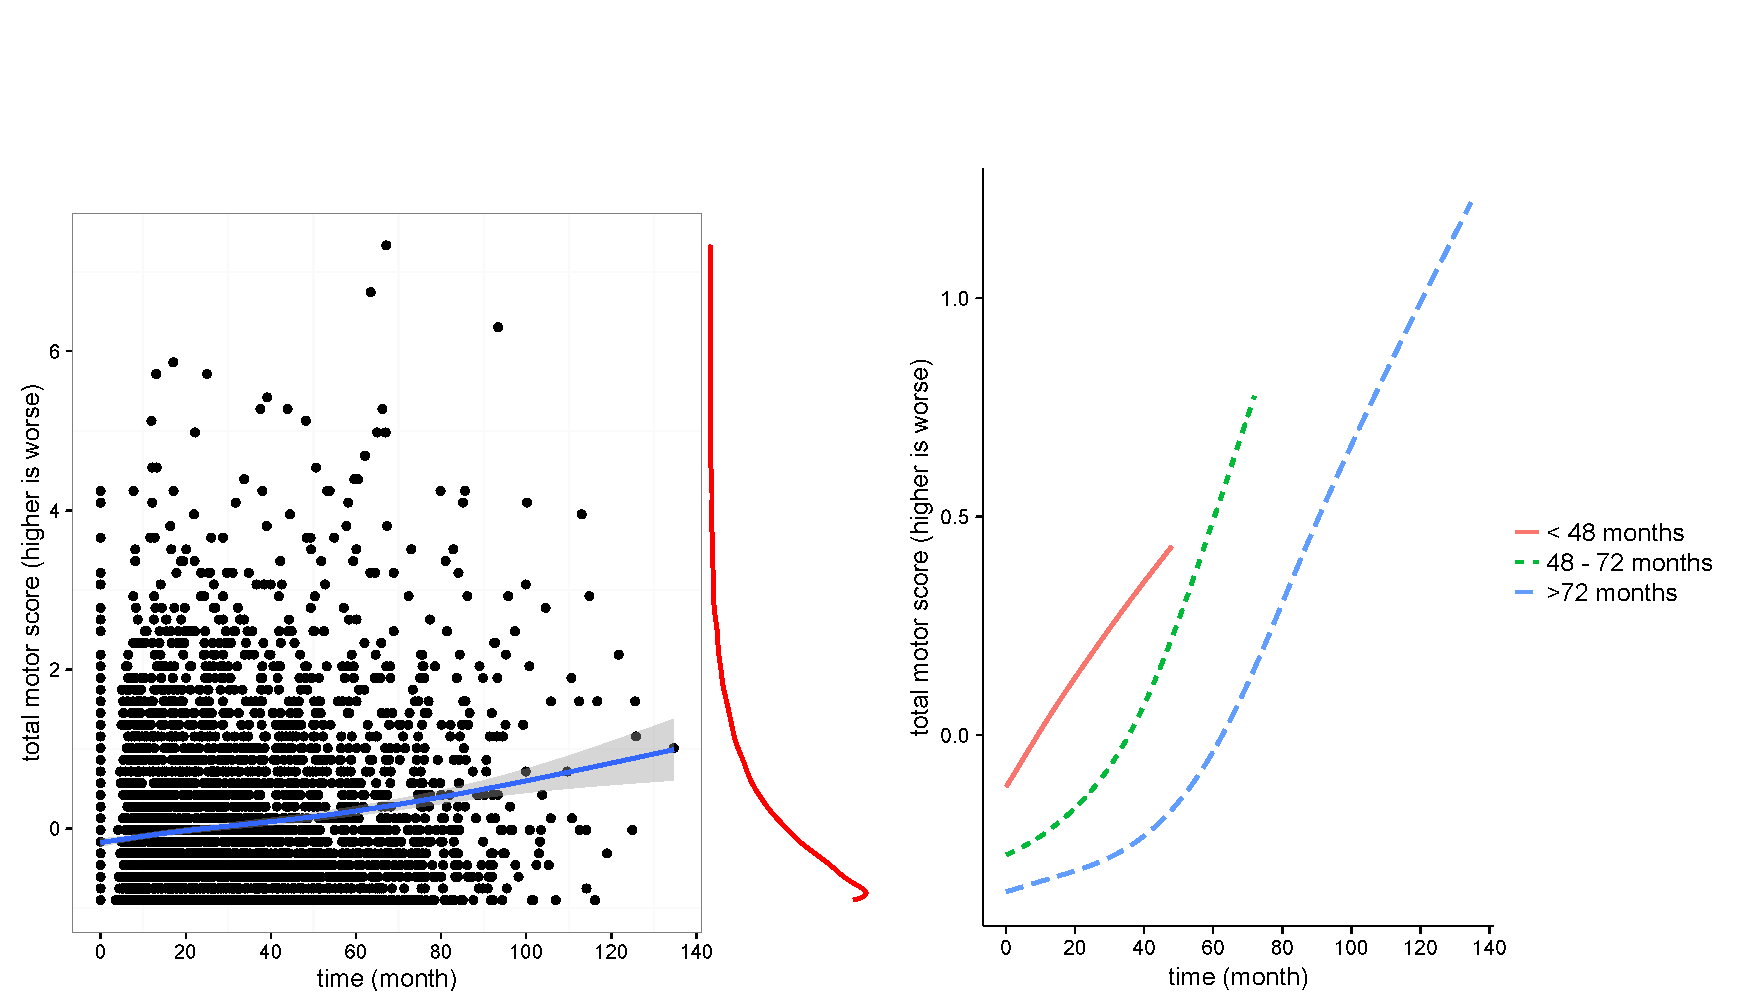
\includegraphics[scale=0.35]{TMS_scatter_loess_grp.eps}\vspace{-1pt}
\caption{ Left panel: Scatter plot (with loess curve) and kernel density plot (right side) for total motor score from the study population (time unit: month; lower total motor score is better); right panel: Mean total motor score values over time.}
\end{figure}
\end{center}
}


\subsection{Joint models for longitudinal and time-to-event data} %
\frame{\frametitle{Joint models for longitudinal and time-to-event data}
% \vspace{-2em}
% \begin{center}
% \begin{figure}
% \includegraphics[scale=0.3]{JMidea.png}
% \caption{Rizopoulos, 2014 (online)}
% \end{figure}
% \end{center}
% \vspace{-1.8em}

\begin{itemize}

\item Traditional joint models (JM)
\small{
\begin{equation*}\label{eqn:joint1}
\left\{
\begin{array}{l}
Y_{i}(t) =m_{i}(t)+\varepsilon_{i}(t)= {\boldsymbol X}_{i}^{\top}(t)\boldsymbol{\beta} + {\boldsymbol Z}_{i}^{\top}(t){\boldsymbol u}_i + \varepsilon_{i}(t), \varepsilon_{i}(t)\overset{iid}{\sim} N(0, \sigma^2)\\
h(t|\mathcal{M}_{i}(t), {\boldsymbol W}_i;  \boldsymbol{\gamma}, \alpha) = h_0(t)\exp({\boldsymbol W}_i^{\top}\boldsymbol{\gamma} + \alpha m_{i}(t))
\end{array}
\right.
\end{equation*}
}

\item Linear mixed model (LMM) for the longitudinal outcome
\item Cox proportional hazards model (PHM) for the time-to-event outcome
\item Longitudinal outcome is treated as a time-dependent covariate in the time-to-event submodel
\end{itemize}

}


\frame{\frametitle{Limitations of traditional JM}

\begin{itemize}
\item LMM is sensitive to outliers and deviation of normality
\item The normality assumption cannot be satisfied in many cases (even after applying various outcome transformations)
\item LMM models only the conditional mean of the outcome -- not very meaningful from clinical perspective in some cases
\end{itemize}
}



\subsection{Research Aims} %%%%%%%
% \frame{\frametitle{Research questions}
% \begin{enumerate}
% \item How to deal with the non-normality in the data?
% \item How to study the covariates effect on the higher/lower tail of the biomarkers?
% \item How to predict event risk in the future? Dynamically?
% \end{enumerate}
% }




\frame{\frametitle{Research aims}
\begin{itemize}
\item {\bf Aim 1}: To build a new JM framework for longitudinal and {\bf survival data} that is more robust against non-normal data and to develop fully Bayesian inference and dynamic prediction algorithms for the proposed JM
\item {\bf Aim 2}: To extend the new JM to study longitudinal data and {\bf recurrent events}, develop a Bayesian method for model inference
\item {\bf Aim 3}: To make dynamic predictions of {\bf recurrent events} risk from the JM developed in Aim 2.
\end{itemize}
}


%%%%%%%%%%%%%%%%%==Aritcles==%%%%%%%%%%%%%%%%%%%%%%%%
\section{Proposed Journal Articles}
%%%%%%%%%%%%%%%%%==Aritcle Two==%%%%%%%%%%%%%%%%%%%%%%%%
\subsection{Journal Article 1}
\frame{\frametitle{Journal Article 1}
\title {Bayesian quantile regression joint models: inference
and dynamic predictions}
\date{}
\maketitle
}

% \subsubsection{Background} %%%%%%%
% \frame{\frametitle{Background}

% \begin{itemize}
%   \item JM: Both longitudinal and survival processes are outcomes of interest; also, the association between the outcomes
%   \item Higher or lower tails of the longitudinal outcome is more relevant to clinical interest compared with conditional mean
%   \item Possible violation of normality assumption of the LMM in traditional JM
%   \item Predictions of future event risk plays an important role in disease intervention and prevention
% \end{itemize}
% }

\subsubsection{Methods} %%%%%%%

\frame{\frametitle{Statistical methods}
\begin{itemize}
\item JM using longitudinal quantile regression
\item Subject-specific dynamic predictions
\end{itemize}

}


\frame{\frametitle{Quantile Regression (QR)}
\begin{itemize}
\item QR models%s a specific quantile of the outcome as a linear function of the covariates:
\begin{equation}\label{eqn:lqr}
Q_{Y|{\boldsymbol X}}(\tau)={\boldsymbol X}^{\top}\boldsymbol{\beta}_{\tau},
\end{equation}
where the $\tau$th quantile of a random variable $Y$, $\tau\in[0,1]$, is defined as
\begin{equation*}\label{eqn:quantile}
Q_{Y}(\tau)=F_{Y}^{-1}(\tau)=\inf\left\{ y:Pr(Y\le y)\geq\tau\right\}.
\end{equation*}

\item Regression parameters are estimated as:
\begin{equation}\label{eqn:loss_fun}
\hat{\boldsymbol{\beta}}_{\tau}=\underset{\boldsymbol{\beta}\in \mathbb{R}^{p}}{\mbox{arg min}}\sum_{i=1}^{n}\left[\rho_{\tau}(Y_{i}-{\boldsymbol X}_i^{\top}\boldsymbol{\beta}_{\tau})\right],
\end{equation}
where $\rho_{\tau}(Y)=Y(\tau-{I}{(Y<0)}).$
%\item There is no direct solution for Equation (\ref{eqn:loss_fun}), and linear programming method can be used to solve it.
\end{itemize}

}


\frame{\frametitle{Parameter estimation from QR vs. mean regression}
\begin{center}
\begin{figure}
\includegraphics[scale=0.45]{MAP.pdf}
\caption{Quantile effect v.s. mean effect}
\end{figure}
\end{center}
}


\frame{\frametitle{Longitudinal quantile regression}
\begin{itemize}
\item The linear quantile mixed model (LQMM):
\[
\left\{
\begin{array}{l}
Y_{i}(t)={\boldsymbol X}_{i}^{\top}(t) \boldsymbol{\beta}_{\tau}+ {\boldsymbol Z}_{i}^{\top}(t)\boldsymbol{u}_i + \varepsilon_i(t),\ i=1, \cdots, N;\ t=1,\cdots, n_i,\\
Q_{Y_{i}(t)|{\boldsymbol X}_{i}, {\boldsymbol Z}_{i}, \boldsymbol{u}_i}(\tau) = {\boldsymbol X}_{i}^{\top}(t) \boldsymbol{\beta}_{\tau}+ {\boldsymbol Z}_{i}^{\top}(t)\boldsymbol{u}_i
\end{array}
\right.
\]\label{eqn:lqmm}

\item Assume asymmetric Laplace distribution (ALD) of the random error, i.e. $\varepsilon_{i}(t)\overset{iid}\sim $ ALD$(0, \sigma, \tau)$:
\begin{equation*}\label{eqn:ald}
f(\varepsilon_{i}(t)|\mu, \sigma, \tau)=\frac{\tau(1-\tau)}{\sigma}\exp\left[-\rho_{\tau}\left(\frac{\varepsilon_{i}(t)}{\sigma}\right)\right];
\end{equation*}

\item Then $Y_{i}(t)|{\boldsymbol X}_{i}, {\boldsymbol Z}_{i}, \boldsymbol{u}_i\overset{iid}\sim$ ALD(${\boldsymbol X}_{i}^{\top}(t)\boldsymbol{\beta}+{\boldsymbol Z}_{i}^{\top}(t)\boldsymbol{u}_i, \sigma, \tau$):

\begin{equation*}\label{eqn:ald_lqmm}
f(Y_{i}(t)|{\boldsymbol X}_{i}, {\boldsymbol Z}_{i}, \boldsymbol{u}_i;\boldsymbol{\beta},\sigma)=\frac{\tau(1-\tau)}{\sigma}\exp\left[-\rho_{\tau}\left(\frac{Y_{i}(t)-{\boldsymbol X}_{i}^{\top}(t)\boldsymbol{\beta}-{\boldsymbol Z}_{i}^{\top}(t)\boldsymbol{u}_i}{\sigma}\right)\right].
\end{equation*}

\end{itemize}
}



\frame{\frametitle{ALD vs. LD vs. Normal}
In ALD($\mu, \sigma, \tau$), $\mu\in(-\infty, \infty)$ is the location parameter, $\sigma$ is the scale parameter and $\tau\in(0, 1)$ is the parameter that control the skewness of the distribution.

\begin{center}
\begin{figure}
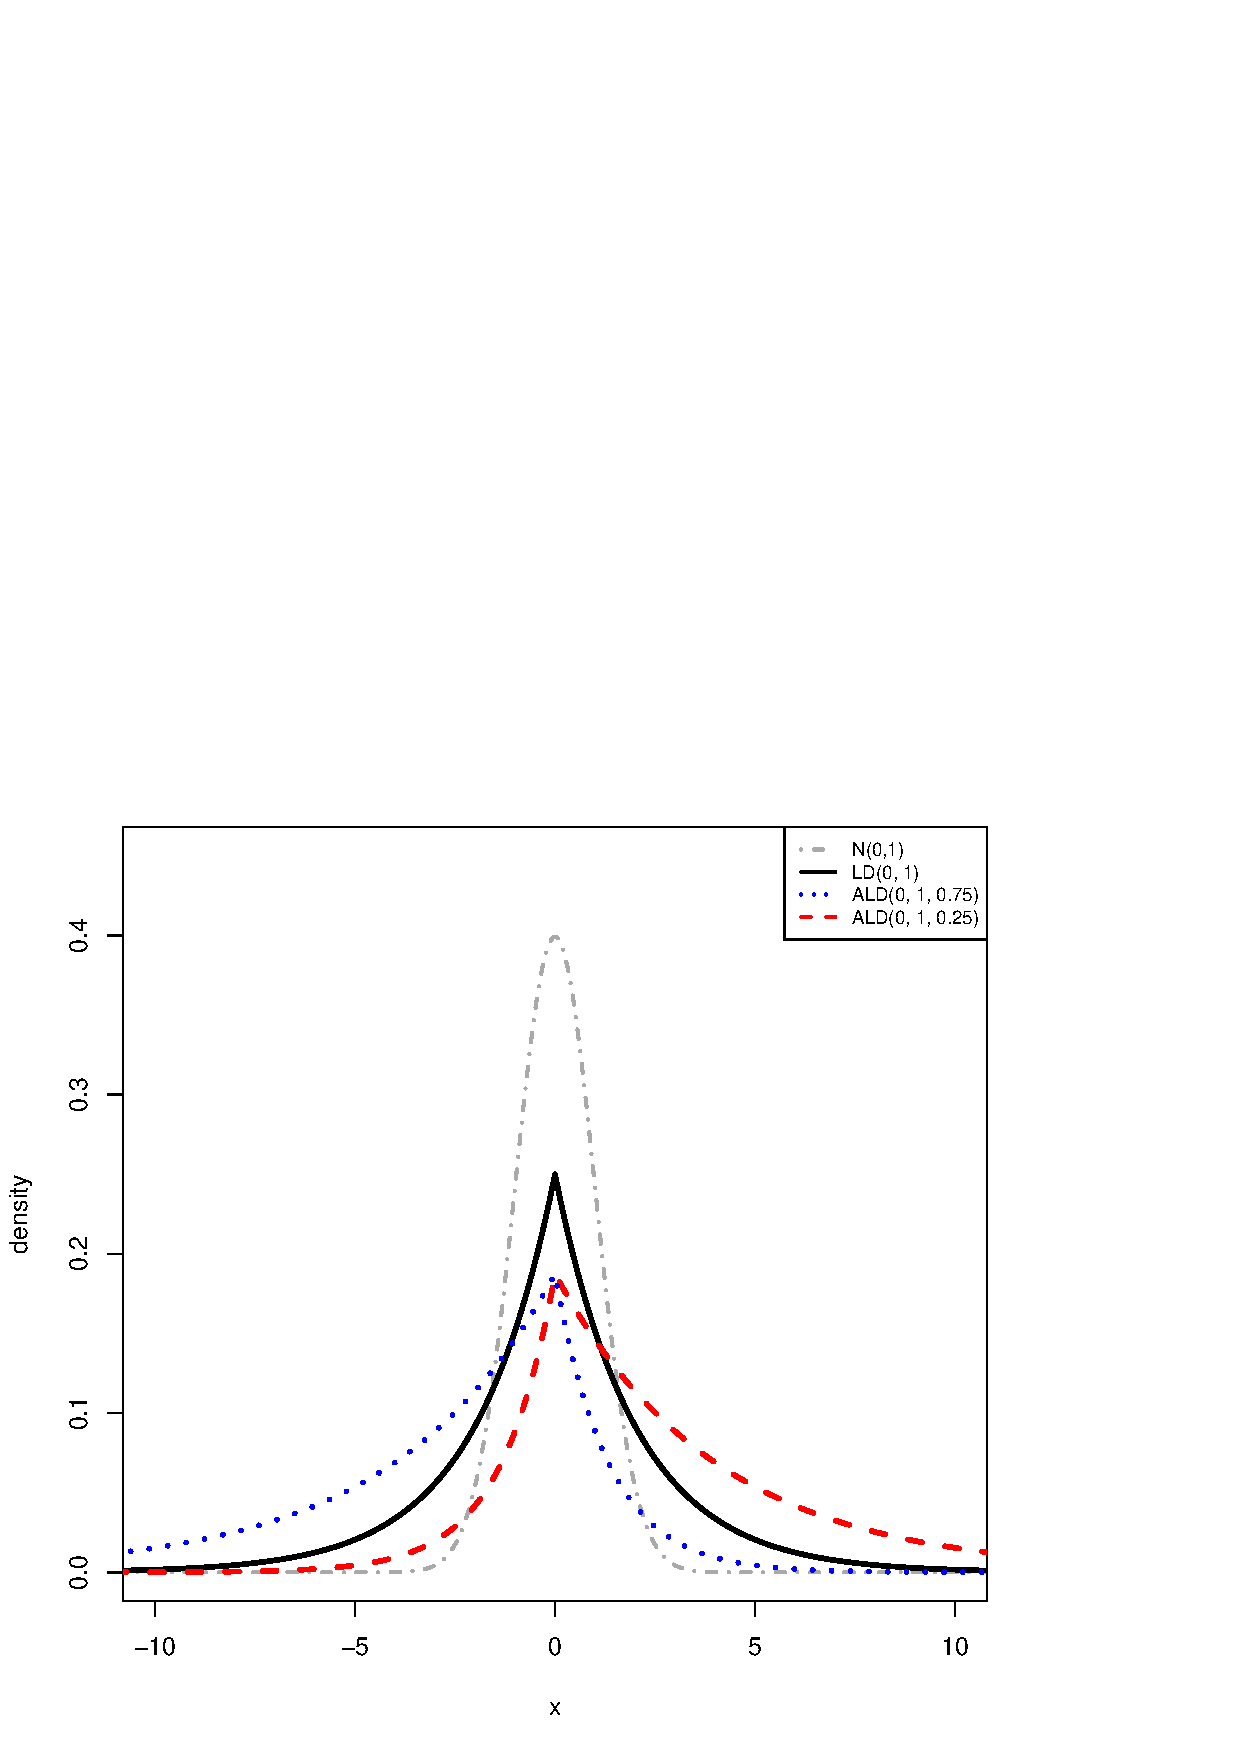
\includegraphics[scale=0.35]{ald_ld_normal.pdf}\vspace{-2pt}
\caption{Asymmetric Laplace, Laplace, and normal distributions}
\end{figure}
\end{center}
}



% \frame{\frametitle{Reparametrization of ALD}
% \begin{itemize}
% \item The location-scale mixture representation of the ALD (Kotz et al., 2001):

% \[\varepsilon_{ij}=\kappa_1e_{ij}+\kappa_2\sqrt{\sigma e_{ij}}v_{ij}.\]

% \item Then the model becomes:
% \begin{equation}\label{eqn:reformald2}
% Y_{ij}={\boldsymbol X}_{ij}^{\top}\boldsymbol{\beta}+{\boldsymbol Z}_{ij}^{\top}\boldsymbol{u}_i+\kappa_1e_{ij}+\kappa_2\sqrt{\sigma e_{ij}}v_{ij}.
% \end{equation}

% where
% \[\kappa_1=\frac{1-2\tau}{\tau(1-\tau)}, \kappa_2^2=\frac{2}{\tau(1-\tau)},\]
% and \[v_{ij}\sim N(0,1), e_{ij}\sim\exp(1/\sigma).\]

% \end{itemize}
%   }



\frame{\frametitle{Quantile regression joint models (QRJM)}
{\small
\begin{equation}\label{eqn:QRJM}
\left\{
\begin{array}{l}
Y_{i}(t) = m_{i}(t) + \varepsilon_{i}(t) = {\boldsymbol X}_{i}^{\top}(t)\boldsymbol{\beta}_{\tau} + {\boldsymbol Z}_{i}^{\top}(t){\boldsymbol u}_i + \varepsilon_{i}(t), \varepsilon_{i}(t)\sim ALD(0, \sigma, \tau)\\
h(T_i|\mathcal{M}_{i}(T_i), {\boldsymbol W}_i;  \boldsymbol{\gamma}_{\tau}, \alpha_{\tau}) = h_0(T_i)\exp({\boldsymbol W}_i^{\top}\boldsymbol{\gamma}_{\tau} + \alpha_{\tau}({\boldsymbol X}^{\top}_{i}(T_i)\boldsymbol{\beta}_{\tau} + {\boldsymbol Z}^{\top}_{i}(T_i){\boldsymbol u}_{i}))
\end{array}
\right.
\end{equation}
}

% where:
\begin{itemize}
\item $m_i(t)$: the error-free longitudinal measure; $\mathcal{M}_{i}(T_i)=\{m_i(s): 0\le s\le T_i\}$
\item $T_i=\min(T_i^*, C_i)$: the event time for subject $i$, where $T_i^*$ is the true underlying event time and $C_i$ is the censoring time
\item $\boldsymbol{\beta}, \boldsymbol{\gamma}$: the fixed effects
\item $\boldsymbol{u}_i$: a vector of random effects for subject $i$
\item $\alpha$: the parameter governing the strength of association
\end{itemize}
}


% \subsubsection{Dynamic predictions of event-free probability}%%%%%%%%%%
\frame{\frametitle{Dynamic predictions of future event-free probability}
\begin{itemize}
\item The predicted probability of no event until time $m$ given no event until time $t$ $(t<m)$ is given by

{\small
\begin{eqnarray}\label{eqn:surv_prob_derv}
&&\nonumber Pr(T_i^*\ge m|T_i^*>t, \mathcal{Y}_i(t), \mathcal{D}_N;\boldsymbol{\theta})\\
&=&\int\frac{{S}_i[m|\mathcal{M}_i(m, u_i, \boldsymbol{\theta});\boldsymbol{\theta}]}{{S}_i[t|\mathcal{M}_i(t, u_i, \boldsymbol{\theta});\boldsymbol{\theta}]}Pr(u_i|T_i^*>t, \mathcal{Y}_i(t);\boldsymbol{\theta})du_i,
\end{eqnarray}}

\item Notations:
\begin{itemize}
\item $p_i(m|t) = Pr(T_i^*\ge m|T_i^*>t, \mathcal{Y}_i(t), \mathcal{D}_n;\boldsymbol{\theta})$: the probability that patient $i$ is free of event up to time $m>t$, given he/she is free of event until time $t$
\item $\mathcal{Y}_i(t)=\{Y_i(s), 0\le s\le t\}$: complete history of observed longitudinal outcome for patient $i$ up to time $t$
\item $\mathcal{D}_N=\{T_i, \Delta_i, \boldsymbol{Y}_i, i=1, \cdots, N\}$: the training data
\end{itemize}
\end{itemize}
}


\frame{\frametitle{Estimation of the predicted probability}
{\small
\begin{itemize}
\item A Monte Carlo (MC) approximation of $p_i(m|t)$ can be obtained using the following procedure:
\begin{enumerate}
\item Draw $\boldsymbol{\theta}^{(p)} \sim Pr(\boldsymbol{\theta}|\mathcal{D}_N)$ for $p=1, \cdots, P$;
\item For each $\boldsymbol{\theta}^{(p)}$, draw ${\boldsymbol u}^{(q)}_i\sim f({\boldsymbol u}_i|T_i^*>t, \mathcal{Y}_{i}(t), \boldsymbol{\theta}^{(p)})$ for $q=1, \cdots, Q$ and compute $$p_i^{(p)}(m|t)=\frac{1}{Q}\sum_{q=1}^QS_i[m|\mathcal{M}_{i}(m, \boldsymbol{u}^{(q)}_i, \boldsymbol{\theta}^{(p)});\boldsymbol{\theta}^{(p)}]S_i[t|\mathcal{M}_{i}(t, \boldsymbol{u}^{(q)}_i, \boldsymbol{\theta}^{(p)});\boldsymbol{\theta}^{(p)}]^{-1};$$
\item Approximate $p_i(m|t)$ by $\hat{p}_i(m|t)=\frac{1}{P}\sum_{p=1}^P p^{(p)}_i(m|t)$ after collecting all $P$ samples of $p_i(m|t)^{(p)}$.
\end{enumerate}
\end{itemize}
}
}


\frame{\frametitle{Predictive accuracy}
\begin{itemize}
\item Let $\hat{r}_i(t+\Delta t | t) = 1- \hat{p}_i(t+\Delta t| t), i = 1, \cdots, N,$ i.e. the event risk.

\item
\begin{equation*}\label{est_TPR}
\widehat{TPR}_{t}^{\Delta t}(c) = \frac{\sum_{i=1}^{N}\hat{r}_i(t+\Delta t|t)I(\hat{r}_i(t+\Delta t|t)\ge c)}{\sum_{i=1}^{N}\hat{r}_i(t+\Delta t|t)},
\end{equation*}
\begin{equation*}\label{est_FPR}
\widehat{FPR}_{t}^{\Delta t}(c) = \frac{\sum_{i=1}^{N}\left(1-\hat{r}_i(t+\Delta t|t)\right)I(\hat{r}_i(t+\Delta t|t)\ge c)}{\sum_{i=1}^{N}\left(1-\hat{r}_i(t+\Delta t|t)\right)}.
\end{equation*}

\item We use the following three statistics as measures of predictive performance (higher is better):

\begin{itemize}
  \item AUC: Area Under (the ROC) Curve
  \item AARD: Above Average Risk Difference
  \item MRD: Mean Risk Difference
\end{itemize}
% \begin{equation*}\label{est_AUC}
% \widehat{AUC}_t^{\Delta t} = \int \widehat{TPR}_t^{\Delta t}\left\{ (\widehat{FPR}_t^{\Delta t})^{-1}(u)\right\}du,
% \end{equation*}

% \begin{equation*}\label{est_AARD}
% \widehat{AARD}_t^{\Delta t} = \widehat{TPR}_t^{\Delta t}(\hat{\rho}) - \widehat{FPR}_t^{\Delta t}(\hat{\rho}),
% \end{equation*}

% \begin{equation*}\label{est_MRD}
% \widehat{MRD}_t^{\Delta t} = \int_c \widehat{TPR}_t^{\Delta t}(c)dc - \int_c \widehat{FPR}_t^{\Delta t}(c)dc,
% \end{equation*}

% \noindent where $\hat{\rho} = \frac{\sum_{i=1}^N \hat{r}_i(t+\Delta t| t)}{N}$ is the average risk in the study population at time $t+\Delta t$.

\end{itemize}
}



%%%%%%%%%%%%%%%%%==SIMULATION==%%%%%%%%%%%%%%%%%%%%%%%%
\subsubsection{Simulation studies} %%%%%%%

% \subsection{Model inference}
\frame{\frametitle{Simulation study I: model inference}
\begin{itemize}
\item Simulate data from QRJM model and consider the following scenarios:
  \begin{enumerate}
  \item Scenario 1: random errors follow ALD(0, 1, $\tau=0.25$) (right-skewed);
  % \item Scenario 2: random errors follow ALD(0, 1, $\tau=0.5$) (symmetric about 0 with heavy tails);
  \item Scenario 2: random errors follow a standard normal distribution (symmetric about 0).
  \end{enumerate}

\item For each scenario, simulate 200 data sets with $N=600$ in each.
\item Among the 600 subjects, randomly select 500 as the training data used to fit the model, and use the remaining 100 subjects as the testing data to make out-of-sample predictions in Simulation II.
\item Compare the bias, standard error (SE), mean squared  error (MSE), and coverage probability (CP) for QRJM and the standard JM (LMJM).
\end{itemize}
}


\begin{frame}[allowframebreaks]
\frametitle{Simulation I results}
\begin{table}[H]
% \begin{center}
\caption{Simulation results in Simulation study I Scenario 1 in which random errors are generated from ALD(0, 1, $\tau=0.25$).}
\adjustbox{max width=\textwidth}{
\label{tab:sim1tab1}
\begin{tabular}{lrcccccccccccccc}
\hline
& \multicolumn{4}{c}{QRJM ($\tau=0.25$)} & & \multicolumn{4}{c}{QRJM ($\tau=0.5$)} & & \multicolumn{4}{c}{LMJM}\\
\hline
 & Bias & SE & MSE & CP && Bias & SE & MSE & CP && Bias & SE & MSE & CP \\
  \hline
  \multicolumn{10}{l}{Coefficients for longitudinal process} \\
  $\beta_0$ & $-$0.003 & 0.080 & 0.014 & 0.930 && 1.659 & 0.129 & 2.807 & 0.020 && 2.702 & 0.146 & 7.350 & 0.000 \\
  $\beta_1$ & 0.015 & 0.068 & 0.010 & 0.950 && 0.024 & 0.105 & 0.043 & 0.890 && 0.080 & 0.116 & 0.052 & 0.860  \\
  $\beta_2$ & 0.016 & 0.083 & 0.013 & 0.950 && 0.014 & 0.112 & 0.042 & 0.970 && 0.078 & 0.128 & 0.052 & 0.920  \\
  \multicolumn{10}{l}{Coefficients for survival process} \\
  $\gamma_1$ & 0.005 & 0.055 & 0.006 & 0.940 && 0.008 & 0.057 & 0.006 & 0.960 && 0.009 & 0.058 & 0.007 & 0.960  \\
  $\gamma_2$ & 0.006 & 0.055 & 0.006 & 0.930 && 0.010 & 0.056 & 0.007 & 0.910 && 0.010 & 0.058 & 0.007 & 0.940  \\
  $\alpha$ & $-$0.004 & 0.078 & 0.010 & 0.970 && $-$0.051 & 0.119 & 0.070 & 0.930 && $-$0.087 & 0.103 & 0.040 & 0.800  \\
   \hline
\end{tabular}
}
% \end{center}
\end{table}

\framebreak
\begin{table}[H]
\centering
\caption{Simulation result in Simulation study I Scenario 2 in which random errors are generated from $\mathcal{N}(0, 1)$.}
\adjustbox{max width=\textwidth}{
\label{tab:sim1tab3}
\begin{tabular}{lccccccccc}
\hline
& \multicolumn{4}{c}{QRJM ($\tau=0.5$)} & & \multicolumn{4}{c}{LMJM} \\
\hline
 & Bias & SE & MSE & CP & & Bias & SE & MSE & CP \\
\hline
  \multicolumn{10}{l}{Coefficients for longitudinal process} \\

  $\beta_0$ & 0.015 & 0.037 & 0.003 & 0.950 & & 0.000 & 0.035 & 0.002 & 0.980 \\
  $\beta_{1}$ & 0.004 & 0.034 & 0.002 & 0.960 & & $-$0.003 & 0.033 & 0.002 & 0.950\\
  $\beta_{2}$ & 0.013 & 0.050 & 0.005 & 0.950 & & 0.006 & 0.049 & 0.005 & 0.950 \\
  \multicolumn{10}{l}{Coefficients for survival process} \\
  $\gamma_1$ & 0.008 & 0.055 & 0.006 & 0.920 & & 0.003 & 0.054 & 0.006 & 0.900 \\
  $\gamma_2$ & 0.015 & 0.055 & 0.007 & 0.920 & & 0.010 & 0.054 & 0.006 & 0.920 \\
  $\alpha$ & $-$0.013 & 0.055 & 0.006 & 0.950 & & 0.007 & 0.055 & 0.006 & 0.950 \\
   \hline
\end{tabular}
}
\end{table}
\end{frame}



% \subsubsection{Dynamic predictions}
\frame{\frametitle{Simulation II: dynamic predictions}
\begin{itemize}
\item Use the 100 subjects as testing data and make out-of-sample predictions
\item Compare the predicted values with the true simulated values (``gold standard'')
\item Use different combinations of $(t, \Delta t)$ for prediction to mimic the real-world situation
\end{itemize}
}


% \begin{frame}[allowframebreaks]
% \frametitle{Simulation II results: Bland Altman plot}
% \begin{figure}[H]
% \centering
% \subfloat[][QRJM with $\tau=0.25$ (True model)]{
%     \includegraphics[width=0.45\columnwidth]{baplot_qt25data_qt25fit_jags_t1.pdf}\label{plot:sim2fig11}
% }
% % \centering
% % \subfloat[][QRJM with $\tau=0.5$]{
% %     \includegraphics[width=0.4\columnwidth]{baplot_qt25data_qt50fit_jags_t1.pdf}\label{plot:sim2fig12}
% % }
% \subfloat[][LMJM]{
%     \includegraphics[width=0.45\columnwidth]{baplot_qt25data_LMJMfit_arms_t1.pdf}\label{plot:sim2fig13}
% }
%   \caption{Bland-Altman plot (bias and 95\% limits of agreement) of gold standard versus model predictions based on the first two longitudinal observations and four different prediction time intervals ($\Delta t_1 < \Delta t_2 < \Delta t_3 < \Delta t_4$) under Scenario 1.}
%   \label{plot:sim2fig1}
% \end{figure}

% \begin{figure}[H]
% \centering
% \subfloat[][QRJM with $\tau=0.5$]{
%     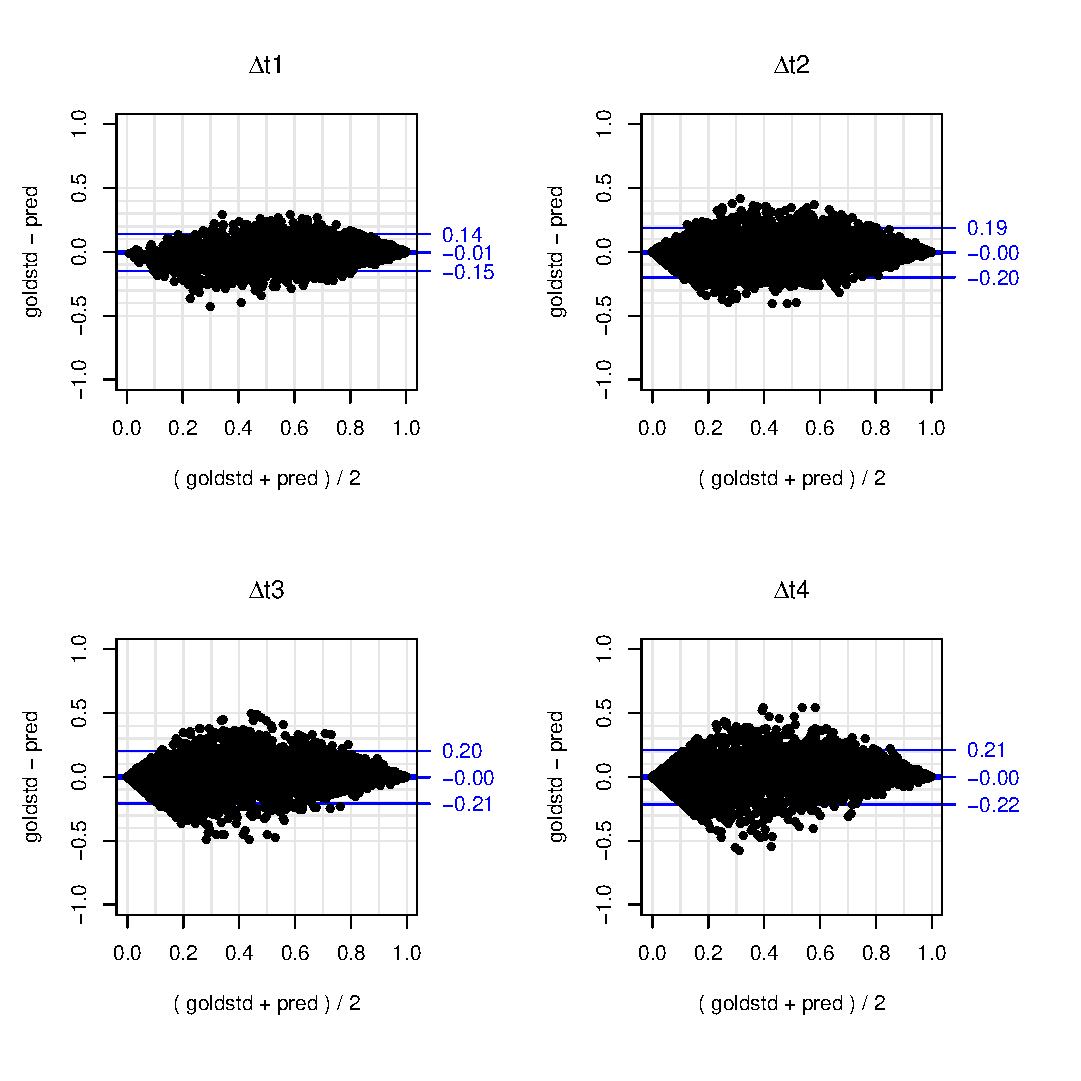
\includegraphics[width=0.45\columnwidth]{baplot_normdata_qt50fit_t1.eps}\label{plot:sim2fig31}
% }
% % \centering
% % \subfloat[][QRJM with $\tau=0.5$]{
% %     \includegraphics[width=0.4\columnwidth]{baplot_qt25data_qt50fit_jags_t1.pdf}\label{plot:sim2fig12}
% % }
% \subfloat[][LMJM (True model)]{
%     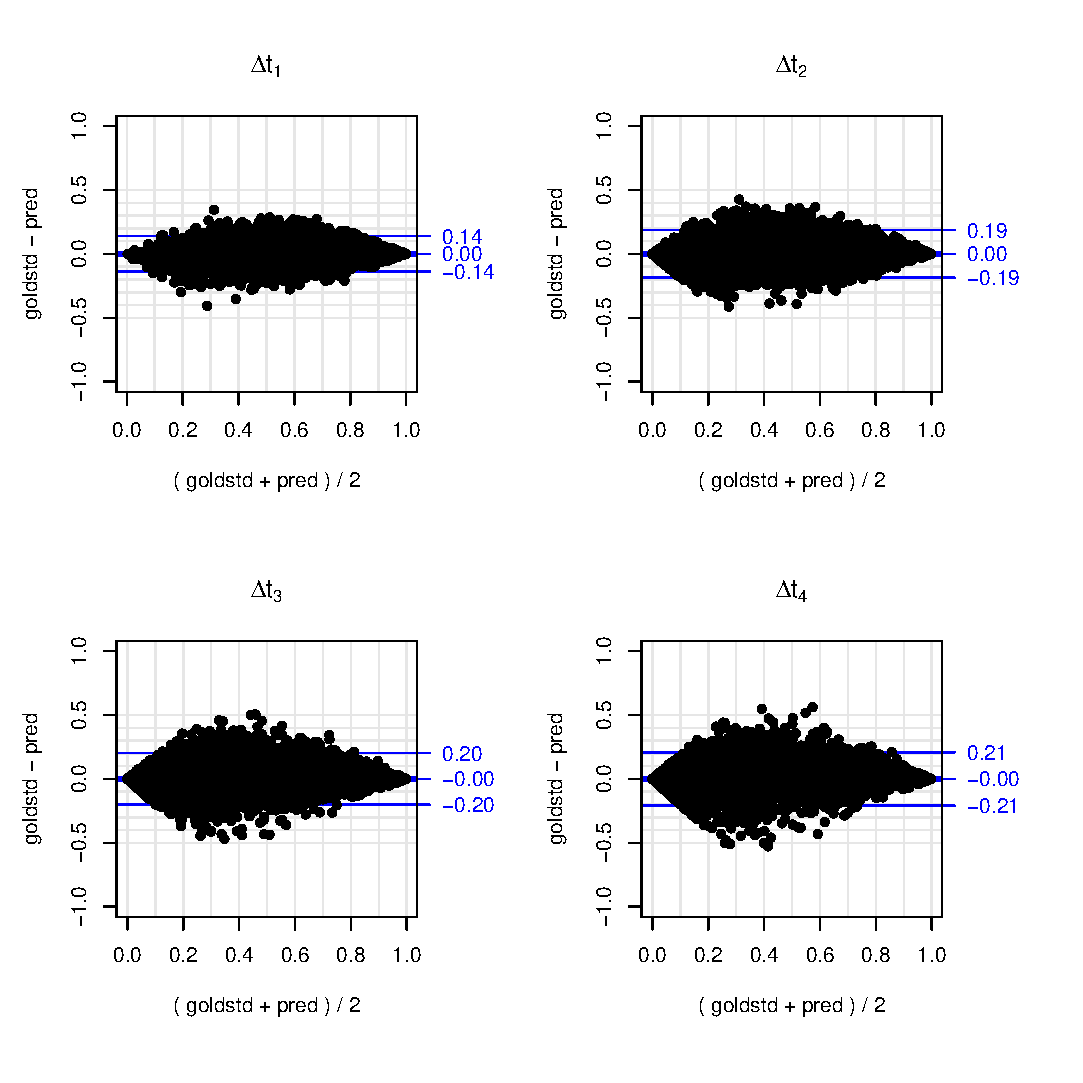
\includegraphics[width=0.45\columnwidth]{baplot_normdata_LMJMfit_t1.eps}\label{plot:sim2fig32}
% }
%   \caption{Bland-Altman plot (bias and 95\% limits of agreement) of gold standard versus model predictions based on the first two longitudinal observations and four different prediction time intervals ($\Delta t_1 < \Delta t_2 < \Delta t_3 < \Delta t_4$) under Scenario 3.}
%   \label{plot:sim2fig2}
% \end{figure}
% \end{frame}



\frame{\frametitle{Simulation II results: summary table}
\begin{table}[H]
\centering
\caption{Simulation result in Simulation study II Scenario 1: MSE and bias of the difference between predicted survival probability and the gold standard.}
\adjustbox{max width=\textwidth}{
\label{tab:sim2tab1}
\begin{tabular}{clcccccccc}
\hline
 & & \multicolumn{2}{c}{QRJM ($\tau=0.25$)} & &\multicolumn{2}{c}{QRJM ($\tau=0.5$)} & &\multicolumn{2}{c}{LMJM} \\
\cline{3-4}\cline{6-7}\cline{9-10}
$t$ & $\Delta t$ & MSE & Bias & & MSE & Bias & & MSE & Bias \\
\hline
\multirow{2}{*}{{\bf 0.25}} & 0.25 & 0.006 & 0.009 && 0.137 & -0.330 & & 0.244 & -0.462 \\
&  1 & 0.010 & 0.007 && 0.111 & -0.267 & & 0.177 & -0.343 \\
\multirow{2}{*}{(subjects left: 48.1\%)} &  2 & 0.012 & 0.003 && 0.083 & -0.197 & & 0.126 &-0.249 \\
&  3 & 0.013 & 0.000 && 0.072 & -0.168 & & 0.107 & -0.210 \\
\hline
\multirow{2}{*}{{\bf 0.5}} & 0.25 & 0.007 & 0.009 && 0.130 & -0.317 & & 0.219 & -0.439 \\
&   1 & 0.015 & 0.000 && 0.144 & -0.321 & & 0.221 & -0.408 \\
\multirow{2}{*}{(subjects left: 34.6\%)}&   2 & 0.017 & -0.015 && 0.121 & -0.259 & & 0.174 & -0.319 \\
&   3 & 0.018 & -0.023 && 0.109 & -0.228 & & 0.153 & -0.278\\
\hline
\multirow{2}{*}{{\bf 0.75}} & 0.25 & 0.009 & 0.005 && 0.125 & -0.301 & & 0.189 & -0.401 \\
& 1 & 0.023 & -0.007 && 0.174 & -0.356 & & 0.253 & -0.447 \\
\multirow{2}{*}{(subjects left: 22.8\%)} & 2 & 0.025 & -0.033 && 0.159 & -0.310 & & 0.218 & -0.375 \\
&  3 & 0.027 & -0.046 && 0.148 & -0.282 & & 0.197 & -0.336\\
\hline
\end{tabular}
}
\end{table}
}


\subsubsection{Application to PREDICT-HD data} %%%%%%%
% \subsection{Data and model}
\frame{\frametitle{Data application}
\begin{itemize}
\item Split the 1078 study participants into two parts: a first sub-cohort of 800 participants is used to draw statistical inference for the unknown parameters; the remainder is used as test data for predictions of HD-free probability.


\item We consider the following joint models for our data analysis:
{\small
\begin{equation*}\label{eqn:data_joint}
\left\{
\begin{array}{l}
y_{i}(t) = m_{i}(t) + \varepsilon_{it} = \beta_0 + \beta_1 t+ \beta_2 age_{0i} + {u}_{i1} + u_{i2} t + \varepsilon_{i}(t),  \varepsilon_{i}(t)\sim ALD(0, \sigma, \tau)\\
h(T_i|\mathcal{M}_{i}(T_i);  \boldsymbol{\gamma}, \alpha) =\lambda(T_i)\exp(\gamma_1 education_i + \gamma_2 I_{male_i} + \alpha m_i(T_i))
\end{array}
\right.
\end{equation*}
}
\item $y_{i}(t)$ represents one of the longitudinal biomarkers
\item $age_0$ is the baseline age at the enrollment.
\item Specify a piecewise constant baseline hazard function with three time intervals, where $\lambda_k$ stands for the hazard rate for time interval $[t_k, t_{k+1})$ and $I_k(t)=1$ if $t\in[t_k, t_{k+1})$ and 0 otherwise.
\end{itemize}
}


% \subsubsection{Results}
\begin{frame}[allowframebreaks]
\frametitle{Data analysis results}
\begin{table}[H]
\centering
\caption{PREDICT-HD data analysis: Parameter estimation and 95\% credible interval from QRJM at three different quantiles with TMS as the longitudinal biomarker.}
\label{realdata_inference}
\adjustbox{max width=\textwidth}{
\begin{tabular}{l ccc }
  % \hline
  % & \multicolumn{3}{c}{{Total Motor Score}}\\
  \hline
  & $\tau=0.25$ & $\tau=0.50$ & $\tau=0.75$ \\
\hline
\multicolumn{4}{c}{\textit{longitudinal TMS process}} \\
int. & -0.760 (-0.903, -0.628)& -0.525 (-0.699, -0.359)& -0.249 (-0.469, -0.035)\\

time (month) & 0.019 (0.015, 0.023)& 0.020 (0.016, 0.024)& 0.022 (0.018, 0.026)\\
$age_0$ & 0.004 (0.001, 0.008)& 0.005 (0.001, 0.010)& 0.006 (0.001, 0.012)\\

\multicolumn{4}{c}{\textit{time to HD onset process}}\\
assoct. & 1.526 (1.321, 1.745)& 1.300 (1.148, 1.459)& 1.080 (0.968, 1.192)\\

eduyr & -0.083 (-0.115, -0.052)& -0.112 (-0.142, -0.082)& -0.128 (-0.157, -0.101)\\

male& 0.317 (-0.037, 0.654)& 0.360 (-0.020, 0.708)& 0.317 (-0.010, 0.647)\\
  \hline
\end{tabular}
}
\end{table}

\vspace{10em}

\begin{table}[H]
\centering
\caption{PREDICT-HD data analysis: AUC, AARD and MRD of the predictions of HD-free probability from QRJM and AUC from LMJM with TMS as the longitudinal biomarker.}
\label{tab:data_auc}
\adjustbox{max width=\textwidth}{
\begin{tabular}{rrrrrrrrrrrrrrc}
\hline
$t$ & $\Delta t$ & \multicolumn{3}{c}{AUC ($\tau$)} & & \multicolumn{3}{c}{AARD ($\tau$)} & & \multicolumn{3}{c}{MRD ($\tau$)} & & \multirow{2}{*}{AUC(LMJM)}\\
\cline{3-5}  \cline{7-9} \cline{11-13}
\multicolumn{2}{c}{(month)}  & 0.25 & 0.50 & 0.75 &  & 0.25 & 0.50 & 0.75&  & 0.25 & 0.50 & 0.75 & & \\
\hline
\multirow{3}{*}{$12$}  & 12 & 0.647 & 0.683 & 0.738 && 0.213 & 0.261 & 0.356 &&  0.010 & 0.020 & 0.059 & &0.679\\
            & 24 &  0.668 & 0.702 & 0.753 &&  0.244 & 0.290 & 0.379 && 0.028 & 0.054 & 0.128 && 0.695\\
            & 36 &  0.685 & 0.714 & 0.760 &&  0.273 & 0.311 & 0.391 && 0.054 & 0.091 & 0.170  & &0.693\\[0.5em]
\multirow{3}{*}{$24$}  & 12 & 0.836 & 0.857 & 0.864  && 0.539 & 0.575 & 0.577 &&  0.168 & 0.218 & 0.285 & &0.855\\
            & 24 &  0.852 & 0.872 & 0.873 && 0.566 & 0.598 & 0.583 && 0.285 & 0.361 & 0.404 & &0.878\\
            & 36 & 0.866 & 0.877 & 0.872 &&  0.581 & 0.599 & 0.575 && 0.368 & 0.420 & 0.430 & &0.836\\[0.5em]
\multirow{3}{*}{$48$}  & 12 &  0.875 & 0.878 & 0.868 &&  0.583 & 0.598 & 0.589 && 0.326 & 0.320 & 0.303 & &0.669\\
            & 24 & 0.875 & 0.883 & 0.874 && 0.578 & 0.602 & 0.598  &&  0.390 & 0.401 & 0.379 & &0.769\\
            & 36 &  0.877 & 0.887 & 0.879 && 0.589 & 0.614 & 0.599  && 0.417 & 0.439 & 0.417 & &0.774\\
\hline
\end{tabular}
}
\end{table}
\end{frame}




\subsubsection{Discussion}
\frame{\frametitle{Discussion}
\begin{itemize}
\item The proposed JM provides a way to explore the covariates effect across the whole distribution span of the outcome variable. This becomes especially important when either the lower or higher quantile of the outcome becomes more relevant to the clinical interest.

\item Our proposed algorithm performs well in recovering the truth in inference and in making predictions of future survival probabilities.

% \item LMJM tended to provide biased point estimates as well as lower coverage probabilities for model parameters when the longitudinal data are skewed.

\item The best predictive performance from our model outperforms that from the LMJM when data are highly skewed.


\item Our novel application of JM in making personalized dynamic predictions of survival probability finds practical importance in many clinical applications.

% \item One possible extension for current model is to incorporate multiple longitudinal biomarkers

\item Predictive accuracy criteria and/or other model selection methods or method(s), e.g. Bayesian model averaging, to incorporate multiple regression results from different quantiles into a single prediction solution can be helpful in selecting the ``best'' quantile in prediction.

\end{itemize}
}



%%%%%%%%%%%%%%%%%==Aritcle Two==%%%%%%%%%%%%%%%%%%%%%%%%
\subsection{Journal Article 2}
\frame{\frametitle{Journal Article 2}
\title {Bayesian Quantile Regression Joint Models of Longitudinal and Recurrent Event Data}
\date{}
\maketitle
}


\subsubsection{Background} %%%%%%%
\begin{frame}[allowframebreaks]
\frametitle{Background}
  \begin{itemize}
    \item Recurrent events are commonly encountered in longitudinal biomedical studies
    \item JM: to simultaneously model the repeated instances of the continuous and time-to-event sequences and to examine the association between the two processes
    \item JM of longitudinal data and recurrent events have received less attention
    \item No work has considered incorporating QR model in JM of longitudinal and recurrent event data so far
  \end{itemize}

  \framebreak
  A simple demo of recurrent events data
  \begin{figure}[H]
  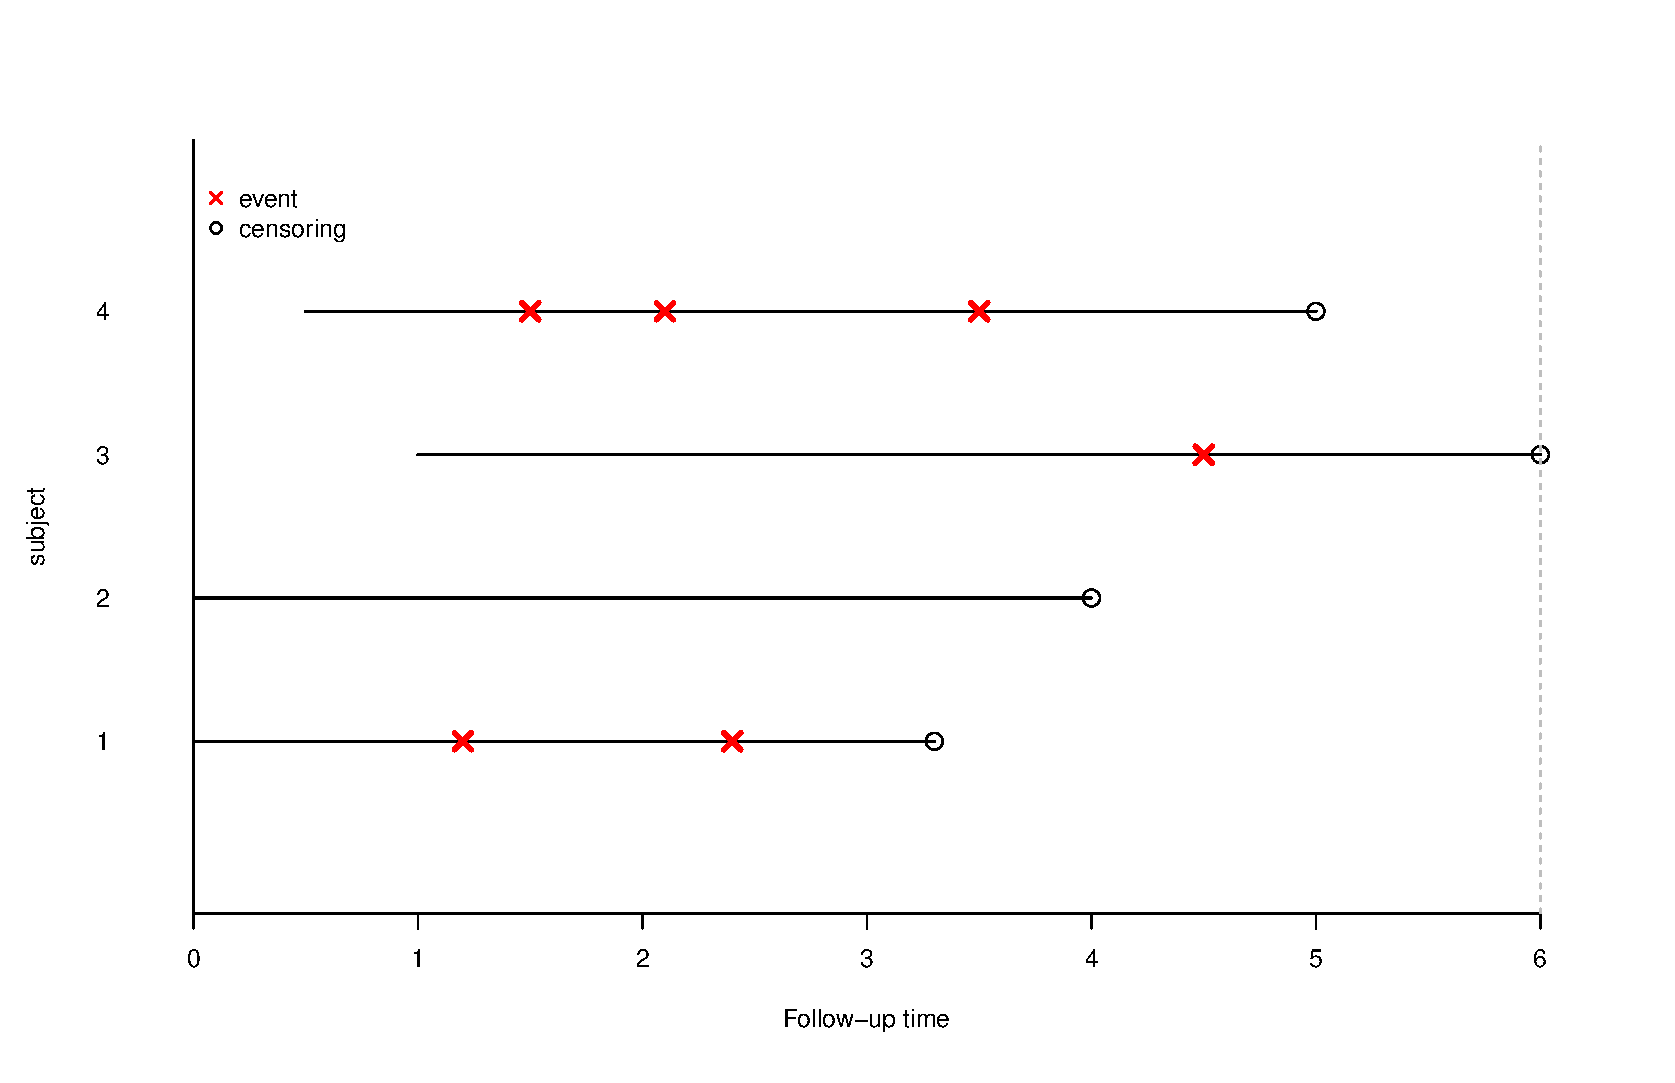
\includegraphics[width=\textwidth]{figures/rec_evt_demo.eps}
  \end{figure}
\end{frame}

\subsubsection{Methods}
\frame{\frametitle{The QRJM}

{\small
\begin{equation}\label{eqn:p2joint}
\left\{
\begin{array}{l}
Y_{i}(t) = m_{i}(t) + \varepsilon_{i}(t) = {\boldsymbol X}_{i}^{\top}(t)\boldsymbol{\beta}_{\tau} + {\boldsymbol Z}_{i}^{\top}(t){\boldsymbol u}_i + \varepsilon_{i}(t), \varepsilon_{i}(t)\sim ALD(0, \sigma, \tau)\\
r_i(t|\mathcal{M}_{i}(t), {\boldsymbol W}_i;  \boldsymbol{\gamma}_{\tau}, \alpha_{\tau}) = r_{i0}(t)\exp({\boldsymbol W}_i^{\top}\boldsymbol{\gamma}_{\tau} + \alpha_{\tau}({\boldsymbol X}^{\top}_{i}(t)\boldsymbol{\beta}_{\tau} + {\boldsymbol Z}^{\top}_{i}(t){\boldsymbol u}_{i}))
\end{array}
\right.
\end{equation}
}
\begin{itemize}
  \item $r_{i0}(\cdot)$ is the subject-specific baseline intensity function
  \item $m_i(t)$ is the true underlying longitudinal outcome at time $t$ and is estimated using an LQMM
  \item $\mathcal{M}_{i}(t)=\{m_{i}(s): 0\le s \le t\}$ is the true longitudinal process up to time $t$
\end{itemize}
}



\frame{\frametitle{Likelihood function of Recurrent events}

Likelihood function for recurrent event data:
{\small
\begin{eqnarray*}\label{eqn:p2lik_sur}
\ell_i({\boldsymbol T}_i, \boldsymbol{\Delta}_i;\boldsymbol{\theta})&=& \nonumber \prod_{k=1}^{m_i}\left[r_i(T_{ik};\boldsymbol{\theta}|\mathcal{M}_{i}(T_{ik}), \boldsymbol{W}_i)^{\Delta_{ik}}\exp\left(-\int_{T_{ik-1}}^{T_{ik}}r_i(s;\boldsymbol{\theta}|\mathcal{M}_{i}(s), \boldsymbol{W}_i)ds\right)\right]\\
&=& \prod_{k=1}^{m_i}\left[r_i(T_{ik};\boldsymbol{\theta}|\mathcal{M}_{i}(T_{ik}), \boldsymbol{W}_i)^{\Delta_{ik}}\right]\exp\left(-\int_0^{T_{im_i}}r_i(s;\boldsymbol{\theta}|\mathcal{M}_{i}(s), \boldsymbol{W}_i)ds\right),
\end{eqnarray*}
}
\begin{itemize}
  \item Let $C_i$ be the censoring time for subject $i$
  \item $m_i$ is the total number of events observed within $C_i$
  \item $T_{ik}$ is the $k$th observed event time, where $k=0, \cdots, m_i$ ($T_{i0}=0$)
  \item $\Delta_{ik} = I(T_{ik} < C_i)$ is the event indicator for $k$th event
\end{itemize}

}


\frame{\frametitle{Complete likelihood and Bayesian inference}
\begin{itemize}
  \item Complete likelihood function for subject $i$
  \begin{equation}\label{eqn:p2full_lik}
  L_i(\boldsymbol{\theta};{\boldsymbol T}_i, \boldsymbol{\Delta}_i, \mathcal{Y}_{i}(C_i), \boldsymbol{u}_i) = \ell_i(\mathcal{Y}_{i}(C_i); \boldsymbol{\theta}|\boldsymbol{u}_i)\ell_i({\boldsymbol T}_i, {\boldsymbol\Delta}_i; \boldsymbol{\theta}|\boldsymbol{u}_i)f(\boldsymbol{u}_i|\boldsymbol{\Sigma})
  \end{equation}

  \item Posterior distributions
  \begin{equation}\label{eqn:p2posterior}
  f(\boldsymbol{\theta}|\boldsymbol{T}, \boldsymbol{\Delta}, \bm{\mathcal{Y}}, \boldsymbol{u})\propto \prod_{i=1}^N L_i(\boldsymbol{T}_i, \boldsymbol{\Delta}_i, \mathcal{Y}_{i}(C_i), \boldsymbol{u}_i;\boldsymbol{\theta}) f(\boldsymbol{\theta})
  \end{equation}

  \[f(\boldsymbol{\theta})=\pi(\boldsymbol{\beta})\pi(\boldsymbol{\gamma})\pi(\alpha)\pi(\sigma)\pi(\boldsymbol{\Sigma})\]

  % \item Prior specification

  % $$\boldsymbol{\beta} \sim \mathcal{N}_p({\boldsymbol 0}, 10^3{\bf I}), \boldsymbol{\gamma} \sim \mathcal{N}_q({\boldsymbol 0}, 10^3{\bf I}), \alpha\sim \mathcal{N}(0, 10^3),$$
  % $$\sigma\sim \mathcal{IG}(10^{-3}, 10^{-3}), \boldsymbol{\Sigma}^{-1}\sim Wishart({\bf I}, k+1). $$

\end{itemize}
}



\subsubsection{Simulation}%%%%%%%%%%%
\frame{\frametitle{Simulation study}
\begin{itemize}
  \item Simulate data from \eqref{eqn:p2joint}, in which the baseline intensity is set to be constant 1
  \item Consider different error distributions:
    \begin{itemize}
    \item Scenario 1: ALD(0, 1, $\tau=0.25$) (right-skewed);
    \item Scenario 2: Standard normal distribution;
    % \item Scenario 3: ALD(0, 1, $\tau=0.50$) (symmetric at 0, heavy tails);
    % \item Scenario 4: ALD(0, 1, $\tau=0.75$) (left-skewed).
    \end{itemize}
  \item For each scenario, simulate 200 data sets with $N = 250$ or 500 in each.
  \item Compare bias, standard error (SE), mean square error (MSE), and coverage probability (CP) for QRJM and the standard JM (LMJM).
\end{itemize}
}

\begin{frame}[allowframebreaks]
\frametitle{Simulation results}

% Tue Oct 27 23:05:22 2015
\begin{table}[H]
\centering
\caption{Simulation result for Scenario 1 in which random error is generated from ALD($0, 1, \tau$ = 0.25).
}
\adjustbox{max width=\textwidth}{
\label{tab:p2simsce1}
\begin{tabular}{clcccccccccccccc}
\hline
& & \multicolumn{4}{c}{QRJM ($\tau=0.25$)} & & \multicolumn{4}{c}{QRJM ($\tau=0.50$)} & & \multicolumn{4}{c}{LMJM}\\
\hline
 & & Bias & SE & MSE & CP && Bias & SE& MSE & CP & & Bias & SE & MSE & CP\\
 \hline
\multirow{9}{*}{$n=250$} &  \multicolumn{12}{l}{Coefficients for longitudinal process}\\
&   $\beta_1$ & 0.014 & 0.091 & 0.008 & 0.980 && 0.025 & 0.102 & 0.012 & 0.960 && 0.036 & 0.112 & 0.013 & 0.955\\
&    $\beta_2$ & $-$0.002 & 0.164 & 0.029 & 0.920 && 0.007 & 0.174 & 0.031 & 0.930 && 0.022 & 0.182 & 0.034 & 0.955\\
&    $\beta_3$ & 0.033 & 0.068 & 0.005 & 0.940 && 0.046 & 0.083 & 0.009 & 0.890 && 0.058 & 0.095 & 0.012 & 0.890\\
&    $\sigma$ & $-$0.000 & 0.031 & 0.001 & 0.950 && $-$0.321 & 0.021 & 0.103 & 0.000 && $-$ & $-$ & $-$ & $-$ \\
&  \multicolumn{12}{l}{Coefficients for recurrent event process}\\
&    $\gamma$ & 0.001 & 0.073 & 0.005 & 0.955 && 0.002 & 0.078 & 0.005 & 0.970 && 0.004 & 0.081 & 0.007 & 0.935\\
&    $r_0$ & 0.032 & 0.134 & 0.018 & 0.945 && $-$0.786 & 0.055 & 0.622 & 0.000 && $-$0.915 & 0.032 & 0.838 & 0.000\\
&    $\alpha$ & $-$0.007 & 0.071 & 0.005 & 0.950 && $-$0.028 & 0.080 & 0.008 & 0.905 && $-$0.030 & 0.090 & 0.009 & 0.920\\
   \hline\hline
\multirow{9}{*}{$n=500$}&  \multicolumn{12}{l}{Coefficients for longitudinal process}\\
&  $\beta_1$ &  $-$0.001 & 0.064 & 0.004 & 0.920 && 0.009 & 0.071 & 0.006 & 0.920 && 0.010 & 0.078 & 0.007 & 0.930\\
&  $\beta_2$ & $-$0.003 & 0.116 & 0.011 & 0.970 & & 0.011 & 0.121 & 0.012 & 0.980 && 0.006 & 0.126 & 0.013 & 0.955\\
&  $\beta_3$ & 0.020 & 0.048 & 0.003 & 0.950 & & 0.026 & 0.058 & 0.004 & 0.950 && 0.029 & 0.067 & 0.005 & 0.935\\
&  $\sigma$ & 0.001 & 0.022 & 0.001 & 0.970 & & $-$0.320 & 0.015 & 0.103 & 0.000 && $-$ & $-$ & $-$ & $-$ \\
&  \multicolumn{12}{l}{Coefficients for recurrent event process}\\
&  $\gamma$ & 0.007 & 0.052 & 0.004 & 0.920 & & 0.007 & 0.056 & 0.004 & 0.920 && 0.007 & 0.058 & 0.004 & 0.915\\
&  $r_0$ & $-$0.017 & 0.093 & 0.008 & 0.940 && $-$0.810 & 0.036 & 0.657 & 0.000 && $-$0.929 & 0.020 & 0.863 & 0.000\\
&  $\alpha$ & 0.003 & 0.051& 0.003 & 0.950 & & $-$0.001 & 0.059 & 0.004 & 0.940 && 0.004 & 0.068 & 0.004 & 0.940\\
   \hline
\end{tabular}
}
\end{table}



\begin{table}[H]
\centering
\caption{Simulation result for Scenario 2 in which random error is generated from $\mathcal{N}(0, 1)$.}
\adjustbox{max width=\textwidth}{
\label{tab:p2simsce4}
\begin{tabular}{clccccccccc}
\hline
& & \multicolumn{4}{c}{LMJM} & & \multicolumn{4}{c}{QRJM ($\tau=0.5$)}\\
\hline
 & & Bias & SE & MSE & CP && Bias & SE & MSE & CP \\
 \hline
\multirow{9}{*}{$n=250$} &  \multicolumn{8}{l}{Coefficients for longitudinal process}\\
  & $\beta_1$ & $-$0.015 & 0.076 & 0.005 & 0.950 && $-$0.010 & 0.076 & 0.006 & 0.960 \\
  &   $\beta_2$ & $-$0.002 & 0.148 & 0.026 & 0.920 && 0.000 & 0.149 & 0.027 & 0.910 \\
  &   $\beta_3$ & 0.004 & 0.038 & 0.001 & 0.970 && 0.003 & 0.038 & 0.002 & 0.920 \\
  &   $\sigma$ & 0.009 & 0.047 & 0.002 & 0.960 &&  $-$ & $-$ & $-$ & $-$ \\
&  \multicolumn{8}{l}{Coefficients for recurrent event process}\\
  &   $\gamma$ & 0.002 & 0.054 & 0.003 & 0.960 && -0.009 & 0.053 & 0.003 & 0.930 \\
  &   $r_0$ & 0.014 & 0.090 & 0.009 & 0.940 && 0.046 & 0.091 & 0.011 & 0.875 \\
  &   $\alpha$ & 0.010 & 0.048& 0.002 & 0.930&& -0.022 & 0.047 & 0.003 & 0.875 \\
   \hline\hline
  \multirow{9}{*}{$n=500$} & \multicolumn{8}{l}{Coefficients for longitudinal process}\\
  & $\beta_1$ &  $-$0.006 & 0.053 & 0.003 & 0.920 && 0.000 & 0.054 & 0.003 & 0.930 \\
  & $\beta_2$ & 0.001 & 0.106 & 0.012 & 0.930 && 0.006 & 0.106 & 0.012 & 0.940 \\
  & $\beta_3$ & 0.010 & 0.026 & 0.001 & 0.920 && 0.009 & 0.027 & 0.001 & 0.920 \\
  & $\sigma$ & 0.003 & & 0.000 & 0.960 &&  $-$ & $-$ & $-$ & $-$ \\
  &  \multicolumn{8}{l}{Coefficients for recurrent event process}\\
  & $\gamma$ & 0.003 & 0.038 & 0.002 & 0.940 && $-$0.007 & 0.037 & 0.002 & 0.930 \\
  & $r_0$ & $-$0.009 & 0.063 & 0.005 & 0.910 && 0.022 & 0.063 & 0.006 & 0.900 \\
  & $\alpha$ & 0.009 & 0.034 & 0.002 & 0.890 && $-$0.014 & 0.033 & 0.002 & 0.850 \\
   \hline
\end{tabular}
}
\end{table}

\end{frame}



\subsubsection{Application to ARIC data}%%%%%%%%
\frame{\frametitle{Data application}
\begin{itemize}
  \item Data from the Atherosclerosis Risk in Communities Study (ARIC).
  \item Longitudinal outcome: systolic blood pressure (SBP); event outcome: coronary heart disease (CHD). Higher SBP leads to higher risk of CHD recurrences (Wattanakit et al., 2005; Rodriguez et al., 2014)
  \item Study cohort: 657 participants; 115, 31, and 17 patients experienced 1, 2 or $\ge 3$ CHD events.
  \item Consider the following QRJM:
    {\small
    \begin{equation*}\label{eqn:p2data_joint}
    \left\{
    \begin{array}{l}
    sbp_{i}(t) = m_{i}(t) + \varepsilon_{i}(t) = \beta_0 + \beta_1 age_{0i} + \beta_2 chol_i + \beta_3 I_{med_i}+ \beta_4 t + {u}_{i1} + u_{i2} t + \varepsilon_{i}(t)\\
    r_i(t|\mathcal{M}_{i}(t);  \boldsymbol{\gamma}, \alpha) = r_0(t)v_i\exp(\gamma_1 I_{male_i} + \gamma_3 I_{smoke_i} + \gamma_4I_{diabetes_i} + \alpha m_i(t))
    \end{array}
    \right.
    \end{equation*}
    }
  \item $r_0(t)$: piecewise constant baseline intensity function with three intervals
  \item $v_i$ is the frailty term that accounts for the correlation among the multiple event times within the same subject
\end{itemize}

}

\begin{frame}[allowframebreaks]
\frametitle{Data analysis results}
% \begin{table}[H]
% \centering
% \caption{ARIC data analysis: Parameter estimation and 95\% credible interval (in parenthesis) from QRJM at five quantiles.}
% \label{p2realdata_inference}
% \resizebox{\linewidth}{!}{
% \begin{tabular}{lccccc}
%   \hline
%   & $\tau=0.05$ & $\tau=0.25$ & $\tau=0.50$ & $\tau=0.75$ & $\tau=0.95$\\
% \hline
% \multicolumn{6}{c}{\textit{longitudinal SBP process}}  \\
%   intercept & $-$0.374 ($-$0.478, $-$0.274) & $-$0.023 ($-$0.118, 0.074) & 0.447 (0.352, 0.554) & 0.872 (0.775, 0.978) &1.187 (1.079, 1.300)\\
%   age$_0$ & 0.035 (0.026, 0.044) & 0.034 (0.025, 0.044) & 0.037 (0.028, 0.047) & 0.040 (0.030, 0.050) & 0.043 (0.031, 0.052)\\
%   total$-$chol.(mg/dL) & $-$0.020 ($-$0.073, 0.033) & $-$0.026 ($-$0.081, 0.032) & $-$0.022 ($-$0.078, 0.037) & $-$0.013 ($-$0.073, 0.047) & $-$0.022 ($-$0.076, 0.032)\\
%   hypertension medicine & $-$0.583 ($-$0.710, $-$0.467) & $-$0.652 ($-$0.773, $-$0.538) & $-$0.725 ($-$0.842, $-$0.609) & $-$0.730 ($-$0.868, $-$0.593) & $-$0.787 ($-$0.924, $-$0.660)\\
%   follow$-$up time (yr) & 0.008 ($-$0.003, 0.018) & 0.006 ($-$0.006, 0.019) & 0.011 ($-$0.001, 0.022) & 0.016 (0.004, 0.029) & 0.019 (0.005, 0.033)\\
%   \multicolumn{6}{c}{\textit{recurrent CHD events process}}  \\
%   association & 0.163 ($-$0.003, 0.332) & 0.207 (0.011, 0.405) & 0.226 (0.019, 0.428) &  0.205 (0.034, 0.374) &0.162 (0.028, 0.288)\\
%   male & 0.191 ($-$0.152, 0.548) & 0.185 ($-$0.170, 0.528) &  0.160 ($-$0.187, 0.507) & 0.132 ($-$0.205, 0.477) & 0.110 ($-$0.234, 0.458)\\
%   ever  smoke & 0.291 ($-$0.044, 0.641) & 0.271 ($-$0.070, 0.613) & 0.216 ($-$0.121, 0.552) & 0.165 ($-$0.177, 0.493) & 0.163 ($-$0.184, 0.485)\\
%   diabetes & 0.918 (0.424, 1.399) & 0.895 (0.409, 1.376) & 0.850 (0.381, 1.349) & 0.811 (0.352, 1.318) & 0.818 (0.333, 1.301)\\
%    \hline
% \end{tabular}
% }
% \end{table}



\begin{table}[H]
\centering
\caption{ARIC data analysis: Parameter estimation and 95\% credible interval (in parenthesis) from QRJM at three quantiles.}
\label{p2realdata_inference}
\resizebox{\linewidth}{!}{
\begin{tabular}{lccc}
  \hline
  & $\tau=0.05$ & $\tau=0.50$ & $\tau=0.95$\\
\hline
\multicolumn{4}{c}{\textit{longitudinal SBP process}}  \\
  Intercept & $-$0.374 ($-$0.478, $-$0.274)  & 0.447 (0.352, 0.554)  &1.187 (1.079, 1.300)\\
  Age$_0$ & 0.035 (0.026, 0.044)  & 0.037 (0.028, 0.047)  & 0.043 (0.031, 0.052)\\
  Total cholesterol (mg/dL) & $-$0.020 ($-$0.073, 0.033) & $-$0.022 ($-$0.078, 0.037) & $-$0.022 ($-$0.076, 0.032)\\
  Hypertension medicine & $-$0.583 ($-$0.710, $-$0.467)  & $-$0.725 ($-$0.842, $-$0.609) & $-$0.787 ($-$0.924, $-$0.660)\\
  Follow-up time (yr) & 0.008 ($-$0.003, 0.018) & 0.011 ($-$0.001, 0.022)  & 0.019 (0.005, 0.033)\\
  \multicolumn{4}{c}{\textit{recurrent CHD events process}}  \\
  Association & 0.163 ($-$0.003, 0.332) & 0.226 (0.019, 0.428)  &0.162 (0.028, 0.288)\\
  Male & 0.191 ($-$0.152, 0.548) &  0.160 ($-$0.187, 0.507)  & 0.110 ($-$0.234, 0.458)\\
  Ever  smoke & 0.291 ($-$0.044, 0.641)  & 0.216 ($-$0.121, 0.552)  & 0.163 ($-$0.184, 0.485)\\
  Diabetes & 0.918 (0.424, 1.399) & 0.850 (0.381, 1.349)  & 0.818 (0.333, 1.301)\\
   \hline
\end{tabular}
}
\end{table}


\begin{figure}[H]
\captionsetup[subfloat]{farskip=1pt,captionskip=1pt}
\centering
\subfloat[Parameters in the longitudinal SBP process]{
    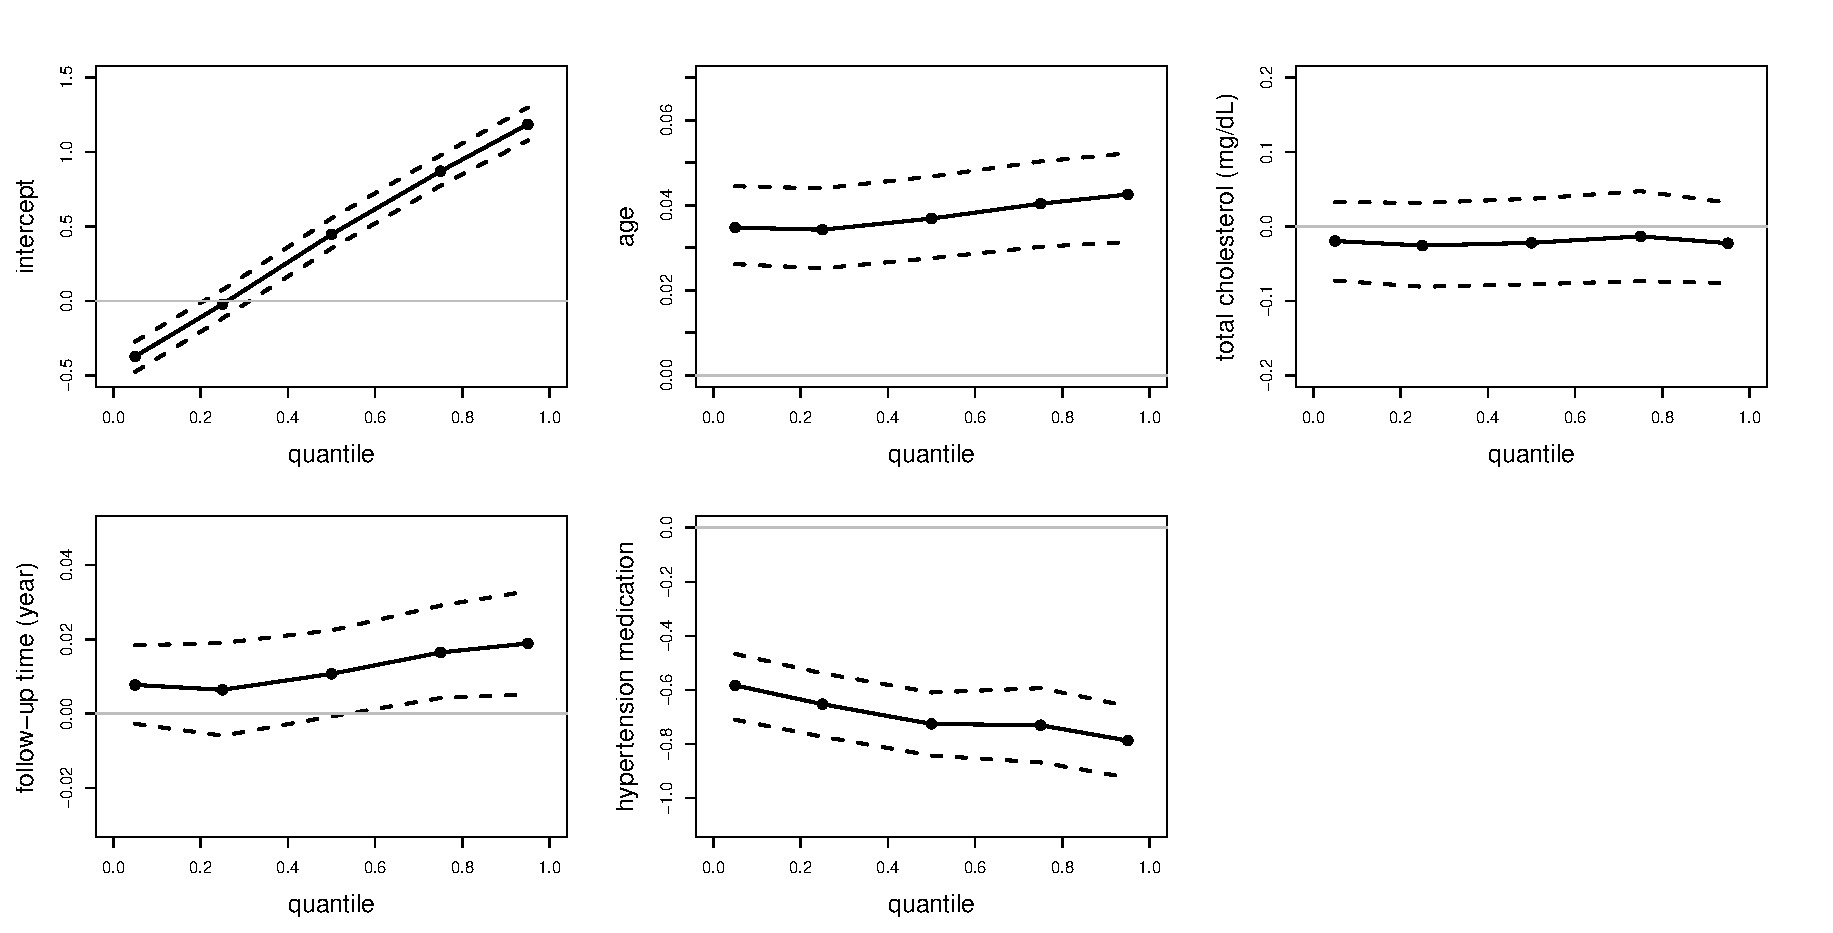
\includegraphics[width=\columnwidth]{figures/p2_JM_inference_covs_long.eps}\label{p2_jm_infer_long}
}

\centering
\subfloat[Parameters in the recurrent CHD events process]{
    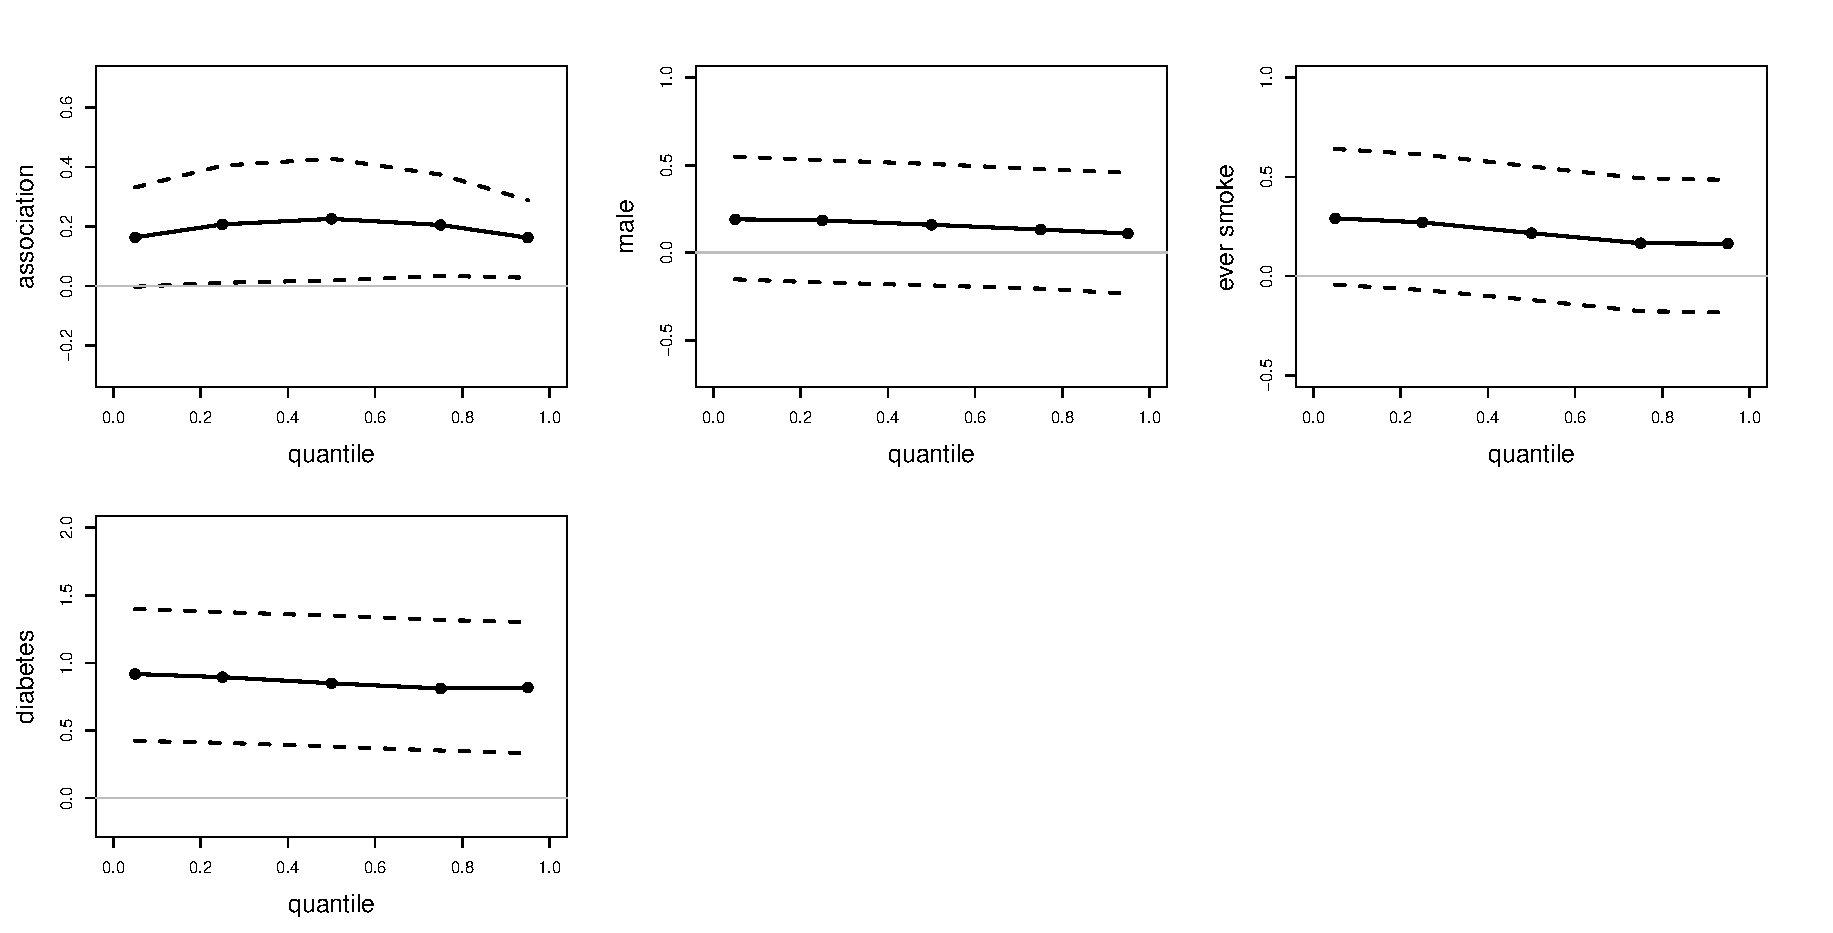
\includegraphics[width=\columnwidth]{figures/p2_JM_inference_covs_rec.eps}\label{p2_jm_infer_rec}
}
  \caption{ARIC data analysis: Posterior mean (solid line) and point-wise 95\% credible interval (dashed lines) of parameter estimation against different quantiles.}
  \label{p2_jm_infer}
\end{figure}

\end{frame}


\subsubsection{Discussion}%%%%%%%%%%%%%%%%%
\frame{\frametitle{Discussion}
\begin{itemize}
  \item Our work on QRJM that uses an LQMM for the longitudinal process provides a more flexible way for simultaneously modeling conditional quantile of a longitudinal outcome and the risk of event recurrences.
  \item In the application of ARIC data our results reveal some findings that can not be observed using linear regression based method.
  \item Our novel extension of traditional JM finds practical importance in many clinical fields: cancer recurrences, hospital readmissions, etc.
  \item Other modeling format consideration: (i) nonlinear QR (Koenker and Park, 1996);  (ii) accelerated failure time model when the proportionality assumption is violated.
\end{itemize}

}



%%%%%%%%%%%%%%%%%==Aritcle Three==%%%%%%%%%%%%%%%%%%%%%%%%
\subsection{Journal Article 3}
\frame{\frametitle{Journal Article 3}
\title {Bayesian Quantile Regression Joint Models: Dynamic Predictions of Recurrent Event Probability}
\date{}
\maketitle
}


\subsubsection{Background} %%%%%%%
\frame{\frametitle{Background}
\begin{itemize}
  \item Disease recurrence is one of the important clinical outcomes in longitudinal biomedical studies.
  \item Accurate predictions of disease probability plays an important role in disease intervention and prevention.
  \item The JM framework offers a novel way of making such personalized dynamic predictions of future event probability (Rizopoulos, 2011; Taylor et al., 2013).
  \item Little work has been done on the dynamic predictions of event recurrences under the JM framework as far, especially the QR based JM
  % \item
\end{itemize}

}

\subsubsection{Methods}
% \frame{\frametitle{Notations}
% \begin{itemize}
%   \item $\mathcal{Y}_{i}(t) = \{Y_i(s): 0\le s \le t\}$ are the observed longitudinal measurements up to time $t$
%   \item $\mathcal{M}_{i}(t)= \{m_i(s): 0\le s \le t\}$ are the true underlying longitudinal measurements up to time $t$
%   \item $\mathcal{T}_{it-}=\{T_{ik}: 1\le k\le K_i, T_{iK_i} < t\}$ are the recurrent times before time $t$
% \end{itemize}
% }


\frame{\frametitle{Predictions of Event-Free Probability}
The predicted event-free probability ($1 - $risk) at time $m$ ($m > t$) given previous event times and longitudinal measurements up to time $t$ is:
\[p_i(m|t) = Pr(T_{iK_i+1}\ge m | T_{iK_i+1}> t, \mathcal{T}_{it-}, \mathcal{Y}_{i}(t); \boldsymbol{\theta}),\]
where $\mathcal{T}_{it-}=\{T_{ik}: 1\le k\le K_i, T_{iK_i} < t\}$ are the recurrent times before time $t$.\\[1em]

With further derivation:
{\scriptsize
\begin{eqnarray}
\label{eqn:p3surv_prob_derv}
p_i(m|t) &=& \int \frac{Pr(T_{iK_i+1}\ge m | \mathcal{M}_{i}(m, \boldsymbol{u}_i; \boldsymbol{\theta}), \mathcal{T}_{it-}; \boldsymbol{\theta})}{Pr(T_{iK_i+1}> t | \mathcal{M}_{i}(t, \boldsymbol{u}_i; \boldsymbol{\theta}), \mathcal{T}_{it-}; \boldsymbol{\theta})}\cdot Pr(\boldsymbol{u}_i|T_{iK_i+1}> t, \mathcal{T}_{it-}, \mathcal{Y}_{i}(t);\boldsymbol{\theta})d\boldsymbol{u}_i
% \nonumber p_i(m|t) &=& \int Pr(T_{iK_i+1}\ge m | T_{iK_i+1}> t, \mathcal{T}_{it-}, \mathcal{Y}_{i}(t), \boldsymbol{u}_i; \boldsymbol{\theta}) \cdot Pr(\boldsymbol{u}_i|T_{iK_i+1}> t, \mathcal{T}_{it-}, \mathcal{Y}_{i}(t);\boldsymbol{\theta})d\boldsymbol{u}_i\\
% \nonumber&=& \int Pr(T_{iK_i+1}\ge m | T_{iK_i+1}> t, \mathcal{T}_{it-}, \boldsymbol{u}_i; \boldsymbol{\theta}) \cdot Pr(\boldsymbol{u}_i|T_{iK_i+1}> t, \mathcal{T}_{it-}, \mathcal{Y}_{i}(t);\boldsymbol{\theta})d\boldsymbol{u}_i\\
% &=&\int \frac{Pr(T_{iK_i+1}\ge m | \mathcal{M}_{i}(m, \boldsymbol{u}_i; \boldsymbol{\theta}), \mathcal{T}_{it-}; \boldsymbol{\theta})}{Pr(T_{iK_i+1}> t | \mathcal{M}_{i}(t, \boldsymbol{u}_i; \boldsymbol{\theta}), \mathcal{T}_{it-}; \boldsymbol{\theta})}\cdot Pr(\boldsymbol{u}_i|T_{iK_i+1}> t, \mathcal{T}_{it-}, \mathcal{Y}_{i}(t);\boldsymbol{\theta})d\boldsymbol{u}_i.
\end{eqnarray}
}

We approximate it by its posterior mean:
\begin{eqnarray}\label{eqn:pexpct_pred}
\nonumber E_{\boldsymbol{\theta}|\mathcal{D}_N}[p_i(m|t)]&=&Pr(T_{iK_i+1}\ge m | T_{iK_i+1}> t, \mathcal{T}_{it-}, \mathcal{Y}_{i}(t))\\
\nonumber &=&\int Pr(T_{iK_i+1}\ge m | T_{iK_i+1}> t, \mathcal{T}_{it-}, \mathcal{Y}_{i}(t); \boldsymbol{\theta})p(\boldsymbol{\theta}|\mathcal{D}_N)d\boldsymbol{\theta}.
\end{eqnarray}
}

\frame{\frametitle{Estimation of the prediction}
A Monte Carlo (MC) estimation of $p_i(m|t)$ can be obtained using the following procedure:
\begin{enumerate}
\item Draw $\boldsymbol{\theta}^{(p)}$ from the posterior distributions $Pr(\boldsymbol{\theta}|\mathcal{D}_N)$ for $p=1, \cdots, P$;
\item For each of the $P$ draws of $\boldsymbol{\theta}^{(p)}$, make $Q$ draws of $\boldsymbol{u}_i^{(q)}, q=1, \cdots, Q$, from the posterior distribution of random effects $Pr(\boldsymbol{u}_i|\mathcal{D}_N, \boldsymbol{\theta}^{(p)})$ and approximate $p_i(m|t)^{(p)}$ by
$$\frac{1}{Q}\sum_{q=1}^Q\frac{Pr(T_{iK_i+1}\ge m | \mathcal{M}_{i}(m, \boldsymbol{u}_i^{(q)}; \boldsymbol{\theta}^{(p)}), \mathcal{T}_{it-}; \boldsymbol{\theta}^{(p)})}{Pr(T_{iK_i+1} > t | \mathcal{M}_{i}(t, \boldsymbol{u}_i^{(q)}; \boldsymbol{\theta}^{(p)}), \mathcal{T}_{it-}; \boldsymbol{\theta}^{(p)})};$$
\item Approximate $p_i(m|t)$ by $\frac{1}{P} \sum_{p=1}^{P} p_i(m|t)^{(p)}$.
\end{enumerate}
}


\subsubsection{Simulation}
\frame{\frametitle{Simulation study}
\begin{itemize}
  \item Simulate data from following JM:
  \begin{equation}\label{eqn:p3simjoint}
  \left\{
  \begin{array}{l}
  Y_{i}(t) = m_i(t) + \varepsilon_{i}(t) = \beta_1X_{1i} + \beta_2X_{2i} + \beta_3t + u_i + \varepsilon_{i}(t)\\
  r_i(t|W_i;  \gamma, \alpha) = r_{0i}(t)\exp(\gamma W_i + \alpha m_i(t))
  \end{array}
  \right.
  \end{equation}

  \item A maximum of six observations for each subject at follow-up times $t =$ 0, 0.25, 0.5, 0.75, 1.0, and 1.25. Also limit a maximum of five recurrent events for each subject.

  \item Consider two scenarios in error distribution: (i) $ALD(0, 1, 0.25)$; (ii) $\mathcal{N}(0, 1)$. 200 data sets for each scenario with $N=$ 500 in each.
  % In the simulated data, around 90\% of the subjects have at least two events.
  % \begin{itemize}
  % \item Scenario 1: $\varepsilon_{i}(t)$ follows ALD with $\tau=0.25$ (right-skewed);
  % \item Scenario 2: $\varepsilon_{i}(t)$ follows standard normal distribution.
  % \item Scenario 3: $\varepsilon_{i}(t)$ follows ALD with $\tau=0.50$ (symmetric at 0, heavy tail);
  % \item Scenario 4: $\varepsilon_{i}(t)$ follows ALD with $\tau=0.75$ (left-skewed);
  % \end{itemize}

\item Split the sample in to two parts: 400 (80\%) are used to draw model inference and the rest 100 subjects are used to make out-of-sample dynamic predictions of event-free probability.
\end{itemize}
}

\begin{frame}[allowframebreaks]
\frametitle{Simulation results}

\begin{table}[H]
\centering
\caption{Simulation result for Scenario 1: MSE and bias of the difference between predicted event-free probability and the gold standard.}
\adjustbox{max width=\textwidth}{
\label{tab:p3sim2qt25data}
\begin{tabular}{clcccccccc}
\hline
 & & \multicolumn{2}{c}{QRJM ($\tau=0.25$)} & &\multicolumn{2}{c}{QRJM ($\tau=0.5$)} & &\multicolumn{2}{c}{LMJM} \\
\cline{3-4}\cline{6-7}\cline{9-10}
$t$ & $\Delta t$ & MSE & Bias & & MSE & Bias & & MSE & Bias \\
\hline
\multirow{2}{*}{{\bf 0.25}} & 0.25 & 0.028 & 0.001 && 0.035 & 0.067 & & 0.033 & 0.023 \\
&  0.50 & 0.035 & $-$0.006 && 0.045 & 0.079 & & 0.043 & 0.024 \\
&  1.00 & 0.037 & $-$0.021 && 0.048 & 0.074 & & 0.046 & 0.015 \\
\hline
\multirow{2}{*}{{\bf 0.5}} & 0.25 & 0.022 & 0.002 && 0.029 & 0.067 & & 0.026 & 0.011 \\
&   0.50 & 0.029 & $-$0.005 && 0.039 & 0.078 & & 0.036 & 0.007 \\
&   1.00 & 0.033 & $-$0.018 && 0.043 & 0.077 & & 0.040 & $-$0.005\\
\hline
\multirow{2}{*}{{\bf 1.00}} & 0.25 & 0.018 & 0.011 && 0.025 & 0.078 & & 0.020 & 0.019 \\
& 0.50 & 0.023 & $-$0.005 && 0.033 & 0.079 & & 0.022 & $-$0.004  \\
&  1.00 & 0.026 & $-$0.016 && 0.036 & 0.078 & & 0.022 & $-$0.009\\
\hline
\end{tabular}
}
\end{table}

% \begin{figure}[H]
% \captionsetup[subfloat]{farskip=-5pt,captionskip=-1pt}
% \centering
% \subfloat[$t = $ 0.25]{
%     \includegraphics[width=\columnwidth]{p3_baplot_qt25data_qt25fit_t1.pdf}\label{plot:p3sim2fig121}
% }

% \centering
% \subfloat[$t=$ 0.50]{
%     \includegraphics[width=\columnwidth]{p3_baplot_qt25data_qt25fit_t2.pdf}\label{plot:p3sim2fig122}
% }

% \centering
% \subfloat[$t=$ 1.00]{
%     \includegraphics[width=\columnwidth]{p3_baplot_qt25data_qt25fit_t3.pdf}\label{plot:p3sim2fig123}
% }
%   \caption{Bland-Altman plot (bias and 95\% limits of agreement) of model predictions versus gold standard based on increasing follow-up time ($t$= 0.25, 0.50, and 1.00) and three different prediction time intervals ($\Delta t1 < \Delta t2 < \Delta t3$) under Scenario 1.}
%   \label{plot:p3sim2qt25_true_pred}
% \end{figure}


\begin{table}[H]
\centering
\caption{Simulation result for Scenario 2: MSE and bias of the difference between predicted event-free probability and the gold standard.}
\adjustbox{max width=\textwidth}{
\label{tab:p3sim2normdata}
\begin{tabular}{clccccc}
\hline
 & & \multicolumn{2}{c}{QRJM ($\tau=0.5$)} & &\multicolumn{2}{c}{LMJM}\\
\cline{3-4}\cline{6-7}
$t$ & $\Delta t$ & MSE & Bias & & MSE & Bias \\
\hline
\multirow{2}{*}{{\bf 0.25}} & 0.25 & 0.015 & $-$0.003 && 0.014 & $-$0.001 \\
&  0.50 & 0.019 & $-$0.007 &&  0.018 & $-$0.003 \\
&  1.00 & 0.020 & $-$0.014 && 0.019 & $-$0.010 \\
\hline
\multirow{2}{*}{{\bf 0.5}} & 0.25 & 0.012 & 0.001 && 0.011 & 0.002 \\
&   0.50 & 0.015 & $-$0.004 && 0.014 & $-$0.002\\
&   1.00 & 0.016 & $-$0.009 && 0.014 & $-$0.007 \\
\hline
\multirow{2}{*}{{\bf 1.00}} & 0.25 & 0.009 & 0.006 && 0.008 & 0.005 \\
& 0.50 & 0.010 & $-$0.004 && 0.009 & $-$0.003 \\
&  1.00 & 0.010 & $-$0.010 && 0.010 & $-$0.009 \\
\hline
\end{tabular}
}
\end{table}
\end{frame}



\subsubsection{Application to ARIC data}
\frame{\frametitle{Data application}
\begin{itemize}
  \item Data from the Atherosclerosis Risk in Communities Study (ARIC).
  \item Longitudinal outcome: systolic blood pressure (SBP); recurrent events: coronary heart disease (CHD).
  \item Select 80\% of the study cohort (i.e. 526 subjects) to draw parameter inference, and make predictions of CHD event probability for the rest 131 individuals.
\end{itemize}
}


\begin{frame}[allowframebreaks]
\frametitle{Dynamic predictions of CHD risk}
\begin{figure}[H]
\centering
\captionsetup[subfloat]{farskip=-3pt,captionskip=0pt}
\subfloat[Predictions based on follow-up time $t = $ 9]{
    \includegraphics[width=\columnwidth, height=0.3\textheight]{qt50_80pct_t9_dt123456.pdf}\label{plot:p3realdata_pred_surv_t9}
}

\centering
\subfloat[Predictions based on follow-up time $t=$ 12]{
    \includegraphics[width=\columnwidth, height=0.3\textheight]{qt50_80pct_t12_dt123456.pdf}\label{plot:p3realdata_pred_surv_t16}
}

\centering
\subfloat[Predictions based on follow-up time $t=$ 14]{
    \includegraphics[width=\columnwidth, height=0.3\textheight]{qt50_80pct_t14_dt123456.pdf}\label{plot:p3realdata_pred_surv_t18}
}
  \caption{ARIC data analysis: Dynamic predictions of CHD event-free probability, based on various follow-up time and prediction time window, with 95\% credible interval from QRJM at $\tau=0.5$ for selected subjects ($*$ indicates CHD event).}
  \label{plot:p3realdata_pred_surv_qt50}
\end{figure}

\framebreak

\begin{table}[H]
\centering
\caption{ARIC data analysis: AUC, AARD and MRD of the predictions of CHD event-free probability from QRJM and AUC from LMJM.}
\label{tab:p3data_auc}
\adjustbox{max width=\textwidth}{
\begin{tabular}{rrrrrrrrrrrrrrc}
\hline
$t$ & $\Delta t$ & \multicolumn{3}{c}{AUC ($\tau$)} & & \multicolumn{3}{c}{AARD ($\tau$)} & & \multicolumn{3}{c}{MRD ($\tau$)} & & \multirow{2}{*}{AUC (LMJM)}\\
\cline{3-5}  \cline{7-9} \cline{11-13}
\multicolumn{2}{c}{(year)}  & 0.25 & 0.50 & 0.75 & & 0.25 & 0.50 & 0.75 & & 0.25 & 0.50 & 0.75 & & \\
\hline
\multirow{3}{*}{$9$}  & 1 & 0.726 & 0.713 & 0.712 && 0.357 & 0.327 & 0.327 &&  0.035 & 0.032 & 0.034 & &0.717\\
            & 2 &  0.685 & 0.671 & 0.670 &&  0.286 & 0.255 & 0.255 && 0.028 & 0.024 & 0.025 && 0.676\\
            & 3 &  0.669 & 0.654 & 0.654 &&  0.257 & 0.227 & 0.228 && 0.027 & 0.022 & 0.023  & &0.659\\[0.5em]
\multirow{3}{*}{$12$}  & 1 & 0.770 & 0.756 & 0.754  && 0.434 & 0.402 & 0.400 &&  0.056 & 0.053 & 0.053 & &0.761\\
            & 2 &  0.721 & 0.703 & 0.703 && 0.345 & 0.303 & 0.304 && 0.044 & 0.039 & 0.039 & &0.710\\
            & 3 & 0.699 & 0.680 & 0.680 &&  0.307 & 0.266 & 0.267 && 0.042 & 0.035 & 0.035 & &0.687\\[0.5em]
\multirow{3}{*}{$14$}  & 1 &  0.797 & 0.784 & 0.784 &&  0.487 & 0.463 & 0.464 && 0.071 & 0.068 & 0.069 & &0.789\\
            & 2 & 0.748 & 0.731 & 0.732  && 0.394 & 0.355 & 0.357  &&  0.059 & 0.054 & 0.054 & &0.738\\
            & 3 &  0.714 & 0.695 & 0.697 && 0.331 & 0.288 & 0.293  && 0.059 & 0.049 & 0.050 & &0.704\\
\hline
\end{tabular}
}
\end{table}
\end{frame}

\subsubsection{Discussion}
\frame{\frametitle{Discussion}
\begin{itemize}
  \item The idea of personalized dynamic predictions of recurrent event risk finds its practical importance in disease control and prevention.
  \item Our novel extension of traditional JM with LQMM adds more flexibility to the modeling framework and allows us to investigate specific subgroup of patients of interest.
  \item  The current version of QRJM uses LQMM and Cox PHM for the longitudinal and recurrent event processes respectively. However, other functional forms for both outcomes can also be considered to extend the proposed method.
  \item The best predictive performance from our model outperforms that from the LMJM. Selection of quantile in prediction or how to combine prediction results from different quantiles can be a topic for future work.
\end{itemize}

}


%%%%%%%%%%%%%%%%%==Acknowledgement==%%%%%%%%%%%%%%%%%%%%%%%%
\section{Acknowledgement} %%%%%%%
\frame{\frametitle{Acknowledgement}
% \vspace{5em},
{\bf Dissertation committee:}\par
Stacia M. DeSantis, PhD (Chair \& Academic Advisor)\par\vspace{0.5em}
Sheng Luo, PhD (Dissertation Supervisor)\par\vspace{0.5em}
David R. Lairson, PhD (Minor Advisor)\par\vspace{0.5em}
Xiaoming Liu, PhD (Breadth Advisor)\\

\vspace{1em}
{\bf External reviewer:}\par
Soeun Kim, PhD


\vspace{2em}
Thanks to all my friends and colleagues at UTSPH and MDACC!

\vspace{2em}
Thanks to the Texas Advanced Computing Center (TACC) for providing high-performing computing resources.

}
%%%%%%%%%%%%%%%%%==Thank you==%%%%%%%%%%%%%%%%%%%%%%%%

\frame{
  \centering
  \begin{figure}
  \includegraphics[width=\textwidth]{figures/Thank_you.jpg}
  \end{figure}
  % {\bf Questions?}
}


%%%%%%%%%%%%%%%%%==References==%%%%%%%%%%%%%%%%%%%%%%%%
\section{References} %%%%%%%
\begin{frame}[allowframebreaks]
\frametitle{Selected references}

\begin{thebibliography}{8}


 \beamertemplatearticlebibitems
  \bibitem{bland1986statistical}
    Bland, J. M. and Altman, D. G.
   \newblock Statistical methods for assessing agreement between two methods of clinical measurement.
    \newblock {\em The Lancet}, 327(8476):307--310, 1986.

 \beamertemplatearticlebibitems
  \bibitem{paulsen2014prediction}
    Paulsen, J. S., Long, J. D., Ross, C. A., Harrington, D. L., Erwin, C. J., Williams, J. K., Westervelt, H. J., Johnson, H. J., Aylward, E. H., Zhang, Y., et al.
    \newblock Prediction of manifest Huntington's disease with clinical and imaging measures: a prospective observational study.
    \newblock {\em The Lancet Neurology}, 13:1193--1201, 2014.


 \beamertemplatearticlebibitems
  \bibitem{kotz2001laplace}
    Kotz, S., Kozubowski, T., and Podgorski, K.
    \newblock The Laplace Distribution and Generalizations: A Revisit With Applications to Communications, Exonomics, Engineering, and Finance.
    \newblock {\em Springer}, 2001.

 \beamertemplatearticlebibitems
 \bibitem{plummerjags}
   Plummer, M. et al.
   \newblock JAGS: A program for analysis of Bayesian graphical models using Gibbs sampling.
   \newblock {\em In Proceedings of the 3rd International Workshop on Distributed Statistical Computing (DSC 2003)}, pages 20--22, March 2003.
%

 \beamertemplatebookbibitems
  \bibitem{koenker2005quantile}
    Koenker, R.
    \newblock Quantile Regression.
    \newblock {\em Cambridge University Press}, 2005.

  \beamertemplatearticlebibitems
  \bibitem{Alessio2014qrjm}
    Farcomeni, A. and Viviani, S.
    \newblock Longitudinal quantile regression in the presence of informative dropout through longitudinal--survival joint models.
    \newblock {\em Statistics in Medicine}, 2015;34(7):1199–1213.



  \beamertemplatearticlebibitems
  \bibitem{rizopoulos2011dynamic}
    Rizopoulos, D.
    \newblock Dynamic Predictions and Prospective Accuracy in Joint Models for Longitudinal and Time-to-Event Data.
    \newblock {\em Biometrics}, 67(3):819--829, 2011.


  \beamertemplatearticlebibitems
  \bibitem{taylor2013real}
    Efendi, A., Molenberghs, G., Njagi, E. N., and Dendale, P.
    \newblock A joint model for longitudinal continuous and time-to-event outcomes with direct marginal interpretation.
    \newblock {\em Biometrical Journal}, 55(4):572--588, 2013.

  \beamertemplatearticlebibitems
  \bibitem{EfendiBJ}
   Taylor, J. M., Park, Y., Ankerst, D. P., Proust-Lima, C., Williams, S., Kestin, L., Bae, K., Pickles, T., and Sandler, H.
    \newblock Real-time individual predictions of prostate cancer recurrence using joint models.
    \newblock {\em Biometrics}, 69(1):206--213, 2013.

  \beamertemplatearticlebibitems
  \bibitem{Wattanakit2005}
  Wattanakit K, Folsom AR, Chambless LE, Nieto FJ.
  \newblock Risk factors for cardiovascular event recurrence in the Atherosclerosis Risk in Communities (ARIC) study.
  \newblock {\em American Heart Journal}. 2005;149(4):606--612.
  \end{thebibliography}
\end{frame}






\end{document}